%=======================================================================
% 中文版前言 — RetNet-0.5B 技术报告
% 编译：在 docs/latex/zh/ 下执行 xelatex 两遍（生成目录与交叉引用）
% 由 mktex.py 的 0p5b 配置引用
%=======================================================================
\documentclass[11pt,openany]{ctexart}

% =====================================================================
%  preamble-common.tex
%  Shared preamble for the RetNet-272M technical report (Chinese and
%  English editions).  Build with XeLaTeX.
%
%  Typographic convention (deliberately plain, single column, as in a
%  conventional technical report):
%    * serif body text, no coloured display headings
%    * numbered tables and figures, each with a caption
%    * remarks set as an indented, labelled passage rather than a
%      coloured box
% =====================================================================

\usepackage{amsmath}
\usepackage{amssymb}
\usepackage{bm}

% ---------- layout ---------------------------------------------------
\usepackage[a4paper,top=2.5cm,bottom=2.5cm,left=2.4cm,right=2.4cm]{geometry}
\usepackage{fancyhdr}
\usepackage{titlesec}
\usepackage{enumitem}
\usepackage{booktabs}
\usepackage{array}
\usepackage{tabularx}
% A table taller than a page must be able to break across pages: an unbreakable
% `tabular` that large is shipped out past the paper edge (Overfull \vbox), and
% the part below the edge is what the reader loses.  `longtable` is used only
% for such tables (see mktex.render_table).
\usepackage{longtable}
\usepackage{ragged2e}
\usepackage{xcolor}
\usepackage{caption}
\usepackage{graphicx}

% ---------- code -----------------------------------------------------
\usepackage{listings}
\usepackage{newunicodechar}

% ---------- references ----------------------------------------------
\usepackage[hidelinks,bookmarksnumbered]{hyperref}
\usepackage{bookmark}

% ---------- colours (used sparingly: code and rules only) ------------
\definecolor{codebg}{RGB}{248,248,249}
\definecolor{codeframe}{RGB}{216,220,225}
\definecolor{codecomment}{RGB}{104,124,108}
\definecolor{codekeyword}{RGB}{0,80,150}
\definecolor{codestring}{RGB}{160,60,40}
\definecolor{rulecol}{RGB}{178,182,188}
\definecolor{headrule}{RGB}{40,48,60}

% ---------- spacing --------------------------------------------------
\linespread{1.04}
\setlength{\parskip}{0.30em}
\setlength{\parindent}{0pt}
\setlength{\abovedisplayskip}{6pt}
\setlength{\belowdisplayskip}{6pt}
\setlength{\abovedisplayshortskip}{4pt}
\setlength{\belowdisplayshortskip}{4pt}

% Mixed CJK / monospace prose has few hyphenation opportunities; give TeX
% more room to stretch instead of leaving overfull boxes.
\tolerance=3000
\emergencystretch=3em
\hyphenpenalty=50
\hbadness=10000

% ---------- headings: plain, black, not coloured ---------------------
\titleformat{\section}
  {\normalfont\large\bfseries}{\thesection}{0.7em}{}
\titleformat{\subsection}
  {\normalfont\normalsize\bfseries}{\thesubsection}{0.7em}{}
\titleformat{\subsubsection}
  {\normalfont\normalsize\itshape}{\thesubsubsection}{0.7em}{}
\titlespacing*{\section}{0pt}{1.5em}{0.55em}
\titlespacing*{\subsection}{0pt}{1.05em}{0.40em}
\titlespacing*{\subsubsection}{0pt}{0.85em}{0.30em}

% ---------- header / footer ------------------------------------------
\pagestyle{fancy}
\fancyhf{}
\renewcommand{\headrulewidth}{0pt}
\renewcommand{\footrulewidth}{0pt}
\fancyfoot[C]{\small\thepage}

% ---------- tables and figures ---------------------------------------
\renewcommand{\arraystretch}{1.18}
\setlength{\tabcolsep}{5pt}
\captionsetup{
  font=small,
  labelfont=bf,
  labelsep=period,
  justification=raggedright,
  singlelinecheck=false,
  skip=5pt,
}
\captionsetup[table]{position=top}
\captionsetup[figure]{position=bottom}

% A numbered table with its caption above, as in the reference report.
\newenvironment{reporttable}[1]
  {\begin{center}\small\captionof{table}{#1}}
  {\end{center}}
\newcommand{\tabnote}[1]{\par\vspace{2pt}{\footnotesize #1}}

% ---------- lists ----------------------------------------------------
\setlist[itemize]{topsep=0.25em,itemsep=0.12em,parsep=0.08em,leftmargin=1.5em}
\setlist[enumerate]{topsep=0.25em,itemsep=0.12em,parsep=0.08em,leftmargin=1.8em}

% ---------- inline code ----------------------------------------------
\newcommand{\code}[1]{\texttt{\small #1}}
\newcommand{\file}[1]{\texttt{\small #1}}

% ---------- code listings --------------------------------------------
\lstdefinestyle{report}{
  backgroundcolor=\color{codebg},
  basicstyle=\ttfamily\fontsize{8.1}{9.6}\selectfont,
  commentstyle=\color{codecomment}\itshape,
  keywordstyle=\color{codekeyword}\bfseries,
  stringstyle=\color{codestring},
  frame=single,
  rulecolor=\color{codeframe},
  framesep=5pt,
  framexleftmargin=5pt,
  xleftmargin=5pt,
  breaklines=true,
  breakatwhitespace=false,
  breakindent=1.2em,
  columns=fullflexible,
  keepspaces=true,
  showstringspaces=false,
  tabsize=4,
  aboveskip=0.6em,
  belowskip=0.6em,
  upquote=true,
  extendedchars=true,
  inputencoding=utf8,
  escapechar=|,
  texcl=false,
  literate=%
    {→}{{$\rightarrow$}}1
    {←}{{$\leftarrow$}}1
    {×}{{$\times$}}1
    {÷}{{$\div$}}1
    {≈}{{$\approx$}}1
    {≤}{{$\leq$}}1
    {≥}{{$\geq$}}1
    {≠}{{$\neq$}}1
    {µ}{{$\mu$}}1
    {γ}{{$\gamma$}}1
    {Δ}{{$\Delta$}}1
    {σ}{{$\sigma$}}1
    {τ}{{$\tau$}}1
    {Σ}{{$\Sigma$}}1
    {√}{{$\surd$}}1
    {·}{{$\cdot$}}1
    {−}{{$-$}}1
    {∈}{{$\in$}}1
    {±}{{$\pm$}}1
    {∞}{{$\infty$}}1
    {❌}{{$\times$}}1
    {✅}{{$\checkmark$}}1
    {⚠}{{!}}1
}
\lstset{style=report}

% `listings` ships no PowerShell dialect; define just enough to colour it.
\lstdefinelanguage{PowerShell}{
  morekeywords={if,else,elseif,foreach,for,while,function,param,return,
    try,catch,finally,switch,break,continue,throw,in,not,and,or},
  sensitive=false,
  morecomment=[l]{\#},
  morestring=[b]",
  morestring=[b]',
}
\lstdefinelanguage{text}{}

% ---------- remarks --------------------------------------------------
% The source uses block quotes for asides.  They are set as an indented
% passage introduced by "Note." rather than as a coloured box.
\newenvironment{notebox}
  {\par\vspace{0.35em}%
   \begin{list}{}{%
     \setlength{\leftmargin}{1.5em}\setlength{\rightmargin}{0.4em}%
     \setlength{\topsep}{0pt}\setlength{\parskip}{0.25em}%
     \setlength{\parsep}{0.25em}\setlength{\itemsep}{0pt}%
     \setlength{\listparindent}{0pt}}%
   \item\relax\textbf{Note.}\ \ignorespaces}
  {\end{list}\vspace{0.15em}}

% ---------- rule -----------------------------------------------------
\newcommand{\reportrule}{\par\vspace{0.5em}{\color{rulecol}\hrule height 0.4pt}\vspace{0.7em}\par}

% ---------- appendices -----------------------------------------------
% The source writes the appendix titles with their letter already in the
% text ("Appendix A: Reproduction"), so the appendix section counter prints
% the letter and the *headings* of the back matter use a second counter that
% renumbers (Reference Reliability Note, References).
\newcounter{backmatter}
\newcommand{\startappendix}{%
  \clearpage
  \setcounter{section}{0}%
  \setcounter{backmatter}{0}%
  \renewcommand{\thesection}{\Alph{section}.}%
  % subsections are numbered against the appendix letter, so pin the format
  % explicitly: leaving \thesubsection as \thesection.\arabic{subsection}
  % would print `B..1' because \thesection already ends in a period.
  \renewcommand{\thesubsection}{\Alph{section}.\arabic{subsection}}%
}
\newcommand{\backmattersection}[1]{%
  \refstepcounter{backmatter}%
  \section*{\arabic{backmatter}.\quad #1}%
  \addcontentsline{toc}{section}{\protect\numberline{\arabic{backmatter}.}#1}%
}


% 中文字体：正文宋体 / 强调黑体 / 引用楷体 / 等宽仿宋
\setCJKmainfont{SimSun}[BoldFont=SimHei,ItalicFont=KaiTi]
\setCJKsansfont{Microsoft YaHei}
\setCJKmonofont{FangSong}

\hypersetup{
  pdftitle  = {RetNet-0.5B：逐段单卡训练到线上的 5.04 亿参数保留网络——宽度生长为何未能解锁},
  pdfauthor = {RetNet 项目组},
  pdfsubject= {保留网络 / 门控线性注意力 / 训练工程 / 推理与服务},
  pdfkeywords={RetNet, GLA, chunkwise, torch.compile, 8-bit AdamW, 0.5B, 单机训练},
}

\begin{document}


%=======================================================================
% 中文版标题页 — RetNet-0.5B
% 标题必须与 docs/26_RetNet-0.5B_技术报告.md 的 H1 一致（H1 不进正文）
% 摘要与目录由 mktex.py 紧随其后插入（摘要取自 Markdown 的 `## 摘要` 一节）
%=======================================================================
\thispagestyle{empty}

\begin{center}
\vspace*{2.6cm}

{\LARGE\bfseries RetNet-0.5B：逐段单卡训练到线上的\\[0.25em] 5.04 亿参数保留网络}

\vspace{0.45cm}

{\large\bfseries ——宽度生长为何未能解锁}

\vspace{0.7cm}

{\small RetNet-0.5B: Training a 504M-Parameter Retentive Network to Production,\\
and Why Width Growth Never Unlocked}

\vspace{0.8cm}

{\normalsize RetNet 项目组}

\vspace{0.25cm}

{\small\itshape 2026-10-13}

\vspace{1.6cm}

{% 表 1 的题注在正文里属于封面块（不进正文），因此手写在这里，编号与正文衔接
\small\textbf{表 1.} 模型摘要（数值出处见正文对应章节）}

\vspace{0.5em}

\begin{minipage}{0.94\textwidth}
\centering\small
\begin{tabular}{@{}rl@{}}
\toprule
模型 & 504.18\,M 参数（504,179,896），20 层，1408 维，22 头 \\
训练 & 三段各一个 epoch，实际消耗 1,656,209,408 token（1.656\,B） \\
硬件 & RTX 3090 24\,GB / RTX PRO 6000 96\,GB / RTX 3070 8\,GB \\
数据 & \code{chat\_pack\_v13}，552,330,489 token 槽位，2048 token 上下文 \\
结果 & 验证 loss 2.6358 $\rightarrow$ 1.9459；生长新增的 82 个仿射张量中 78 个逐位为 0 \\
\bottomrule
\end{tabular}
\end{minipage}

\vfill

{\small\itshape 本 PDF 为中文版；英文版为另一文件 RetNet-0.5B-Technical-Report.pdf。}

\vspace{1.0cm}
\end{center}

\clearpage


\section*{摘要}

\addcontentsline{toc}{section}{摘要}

RetNet 的线性递推让长序列推理的显存与序列长度无关，但也让一个 5 亿参数级的模型只能靠单卡显存和单卡时间预算来推进，本项目的全部设计选择都受这两条约束支配。本报告记录 \code{checkpoints\allowbreak{}/retnet\allowbreak{}\_500m\allowbreak{}\_v15b\allowbreak{}\_ep3} 这一个具体模型从零训练到在线服务的完整工程事实：\textbf{504,179,896} 个参数、20 层、\code{d\allowbreak{}\_model} 1408、22 头，语料是 \code{data\allowbreak{}\_cache\allowbreak{}/chat\allowbreak{}\_pack\allowbreak{}\_v13} 的 \textbf{552,330,489} 个 token 槽位，训练 \textbf{3 段}（ep1 在 RTX 3090 24 GB、ep2/ep3 在 RTX PRO 6000 96 GB，逐段训练、无多卡并行）、三段实际消耗 \textbf{1,656,209,408} token（按名义参数 \textbf{3.28496} token/参数；三个 token 口径的定义与差异见 4.1 节），验证损失从 \textbf{2.6358} 降到 \textbf{1.9459}；同一套权重可以在并行（parallel）、分块（chunkwise）、循环（recurrent）三种等价计算形式之间切换，训练用分块、预填用并行、逐 token 解码用循环。工程侧有三类值得单独记录的发现：一步 575 ms 里有 61.6\allowbreak{}\% 是 GEMM、3.8–4.3\allowbreak{}\% 是可消除的结构性冗余；\textbf{四类不报错的缺陷}（检查点覆盖命令行 batch 与缺 \code{optimizer\allowbreak{}.pt} 时调度器不恢复、\code{\allowbreak{}-\allowbreak{}-eval\allowbreak{}\_batches} 死字段被静默忽略、吞吐字段用 \code{max\allowbreak{}\_steps} 当分子、等价性测试把被测函数当参考）各自有可复现的日志证据；以及一项已由核查员复核的结构性实测——生长新增的 82 个仿射张量里 \textbf{78 个逐位为 0}（4 个反例在 L18/L19），使检查点里 \textbf{67.08\allowbreak{}\%} 的权重元素恰好为零，机制是 \code{gamma\allowbreak{}\_new = 0} 的自锁（2.4 节）。该计数已复核，但\textbf{未做反向传播，因此"非零"不等于"可训练"}。评测与服务的详细结果见第 5、6 章；权重与模型卡发布在 Hugging Face（见第 6 章的部署形态一节）。

\renewcommand{\contentsname}{目录}
\tableofcontents

\clearpage

\section{引言}

本章交代两件事：约束是什么，以及本报告为什么把负面结果放在与正面结果同等的位置。

约束是单卡：8 GB 的 RTX 3070、24 GB 的 RTX 3090、96 GB 的 RTX PRO 6000。参数量的每一次上调都直接换算成显存与墙钟，墙钟再换算成人民币（单价见 4.5 节）。这不是"算力足够、只差调参"的环境：24 GB 线上训练时的显存余量只有 1,346 MiB（23,230 / 24,576 MiB，见 \code{logs\allowbreak{}/gpu\allowbreak{}-host\allowbreak{}\_20261012\allowbreak{}/logs\allowbreak{}/linux\allowbreak{}/\allowbreak{}\_peak\allowbreak{}\_v15b\allowbreak{}\_seg1\allowbreak{}.txt} 的收尾行；同目录的 \code{\allowbreak{}\_peak\allowbreak{}\_v15b\allowbreak{}.txt} 是 23,118 MiB / 余量 1,458 MiB，两者属不同分段，不要混挂同一个余量）；8 GB 线上 0.5B 的余量只有 517 MiB。因此批量、精度、优化器、梯度检查点这几项没有"选最优"的余地，只有"装得下/装不下"。

RetNet（retentive network）用固定的几何衰减代替注意力，于是同一个模型有并行、循环、分块三种数学等价的计算形式：并行训练友好但显存随序列长度平方增长，循环显存恒定但只能逐 token 推进，分块是两者的折中。本报告关心的是这三种形式在同一套权重上能否互换、数值是否等价（2.3 节与 6.1 节）。

本报告\textbf{不提出新架构}。它记录的是一个从零初始化（经由函数保持的宽度生长）、在 RTX 3090 与 RTX PRO 6000 上\textbf{逐段}训练约 16.79 GPU 小时（每段独占单卡，无多卡并行）、在 1,020 项基准上被测量、并以流式接口公开服务的具体模型。之所以值得成文，原因有三条：一是所有性能数字都指得到具体文件与字段，包含被推翻的推算值；二是\textbf{阴性结果与阳性结果同等篇幅}（3.5 节、附录 C），本项目在"改了几行、变快了"和"改了几行、什么也没发生"之间不做取舍；三是本文记录了四类\textbf{不报错的缺陷}（3.4 节），它们都属于同一族：日志看起来正常、数值看起来合理，只有在特定条件下才是错的。

\section{架构}

本章回答"这个模型长什么样"，包括与原始 RetNet 论文的两处偏离，以及其中一处在本代模型里没有生效的实测证据。

\subsection{保留机制}

原始的 RetNet 保留层用按头固定的几何衰减 $\gamma_h$ 为历史加权。并行形式的输出是

\[
\mathrm{Ret}(X)=\big(QK^{\top}\odot D\big)V,\qquad D_{ij}=\gamma_h^{\,i-j}\,[\,i\ge j\,],
\]

循环形式把同一件事写成状态递推，状态尺寸与序列长度无关：

\[
S_n=\gamma_h\,S_{n-1}+k_n v_n^{\top},\qquad o_n=q_n^{\top}S_n .
\]

$\gamma_h$ 就是"每个头记多久"的旋钮：$\gamma_h\to1$ 表示几乎不遗忘，$\gamma_h\to0$ 表示只看当前 token。原始论文取 $\gamma_h=1-2^{-5-h}$，即按头编号几何递减。

\subsection{逐头可学习衰减门}

本实现把 $\gamma$ 从固定公式改成可学习参数（门控线性注意力，gated linear attention，GLA）：\code{retnet\allowbreak{}\_hf\allowbreak{}/modeling\allowbreak{}\_retnet\allowbreak{}.py:98\allowbreak{}-103} 先用 $1-2^{-5-h}$ 初始化，\code{use\allowbreak{}\_gla=true} 时把它注册为 \code{nn\allowbreak{}.Parameter}，否则注册为 buffer。参数\textbf{直接是 $\gamma$，不是 $\log\gamma$}，因此它的取值范围不由参数化保证，训练可以把它推到 1 以上或 0。

这一点在实现上留了两个必须处理的边界。第一，$\gamma$ 必须保存在 fp32：bf16 只有 7 位尾数，在 1.0 附近的 ulp 约 $2^{-8}$，相邻头的衰减会被压成同一个值。本模型 \code{config\allowbreak{}.json} 的 \code{dtype} 是 \code{float32}（该文件没有 \code{torch\allowbreak{}\_dtype} 键），权重文件逐张量读出也全部是 \code{F32}；440 个 $\gamma$ 的实测最小值 0.1999、最大值 0.9985。第二，衰减表的两种写法在 $\gamma$ 的两端各坏一个：因式分解的 $\gamma^{i}\cdot\gamma^{-j}$ 一旦需要 $\gamma^{-255}$ 就溢出 fp32；朴素的 $\gamma^{\delta}$ 对 $\gamma>1$ 不成立。\code{retnet\allowbreak{}\_hf\allowbreak{}/retention\allowbreak{}\_fast\allowbreak{}.py:51\allowbreak{}-92} 因此统一走对数空间 $\exp(\log\gamma\cdot\delta)$，并把 $\gamma$ 夹到一个正下限，使 $\gamma=0$ 处 $\exp(\log\gamma\cdot 0)=1$，与参考实现 $0^0=1$ 的语义一致（\code{retention\allowbreak{}\_fast\allowbreak{}.py:75\allowbreak{}-80}）。

梯度的路径与 $\gamma$ 出现的三处一一对应：并行的 $\gamma^{i-j}$、分块的 \code{inner\allowbreak{}\_mask}/\code{cross\allowbreak{}\_decay}/\code{value\allowbreak{}\_decay}/\code{chunk\allowbreak{}\_decay} 四张表、循环的 $\gamma\cdot S_{n-1}$。$\gamma$ 是一维参数，反向要把 batch、序列、chunk 维度全部归约掉；这一步在计算账里是独立一项（\code{docs\allowbreak{}/25:30}，约 12 GiB/步、约 7 ms）。

本代模型的 $\gamma$ 实测值（\code{checkpoints\allowbreak{}/retnet\allowbreak{}\_500m\allowbreak{}\_v15b\allowbreak{}\_ep3\allowbreak{}/model\allowbreak{}.safetensors}，键 \code{blocks\allowbreak{}.*\allowbreak{}.msr\allowbreak{}.gamma}，20 层 $\times$ 22 头 = 440 个数）：最小值 \textbf{0.1999}、最大值 \textbf{0.9985}、均值 \textbf{0.6997}，\textbf{没有任何头超过 1}。第 3 层前 16 个头逐头不同（0.429 / 0.867 / 0.846 / 0.988 / …），而后 6 个头在\textbf{全部 20 层}里都等于同一个常数 \textbf{0.5430}；第 12–15 头在多数层里同为 0.4462。同一常数跨层重复不是巧合：AdamW 的\textbf{解耦权重衰减}在梯度为 0 时仍会继续缩小参数，

\[
\gamma_{t+1}=\gamma_t\cdot\exp(-\eta_t\,w),
\]

其中 $\eta_t$ 是该步学习率、$w$ 是 \code{weight\allowbreak{}\_decay}。核查员按三段 \code{trainer\allowbreak{}\_state\allowbreak{}.json} 的逐步 \code{learning\allowbreak{}\_rate} 积分得 $\sum_t\eta_t=6.1078$，乘以 $w=0.1$ 得 $\gamma_{\text{pred}}=\gamma_{\text{init}}\cdot\exp(-0.6108)=0.5429$，而实测是 \textbf{0.5430（差 0.02\allowbreak{}\%）}。因此 heads 16–21 的准确表述是：\textbf{从未收到梯度，但被权重衰减推低了约 45.7\allowbreak{}\%}；heads 12–15 的 0.4462 需要额外约 $\sum_t\eta_t\approx1.96$ 的同类衰减才能解释（\textbf{推导}，对应这些头已被零权重切断之后仍在继续的训练）。这两条都是已验证的推论，不是假说，也与 2.4 节的实测结构互为印证。

\subsection{三种计算范式与分块闭式解}

参考实现的分块形式是逐块循环：每块 4 次矩阵乘，外加一次小的状态递推。\code{retnet\allowbreak{}\_hf\allowbreak{}/retention\allowbreak{}\_fast\allowbreak{}.py} 的批量写法把它压成 3 次矩阵乘，关键是观察到块间衰减 $d=\gamma^{C}$ 在循环里是常量，于是"块 i 之前的状态"有闭式解：

\[
S_{\text{prev}}[i]=d^{i}S_0+\sum_{j<i}d^{\,i-1-j}U_j,\qquad U_j=k_j^{\top}\big(v_j\odot\gamma^{\,C-1-\cdot}\big),
\]

它等价于对下三角矩阵 $T_{i,j}=d^{\,i-1-j}\,[\,i-1-j\ge0\,]$ 做一次批量矩阵乘 $S_{\text{all}}=T\,U$。与"对数深度扫描（Hillis–Steele）"的差别在于：$T$ 只有 $H\cdot(nc+1)\cdot nc$ 个元素（$nc=16$、$H=22$ 时是 5,984 个 fp32），不物化任何额外的大张量；而对数深度扫描还要每轮物化一个 \code{[B,H,nc,kd,vd]} 量级的张量（\code{retention\allowbreak{}\_fast\allowbreak{}.py:140\allowbreak{}-147} 记录了这条取舍）。闭式解的所有指数非负，因此不存在 $\gamma^{-j}$ 溢出，$\gamma$ 再小也只是下溢到 0（代表历史被忘光）。

三条路径由 \code{RETNET\allowbreak{}\_FAST\allowbreak{}\_CHUNKWISE=1} 与 \code{mode} 选择，数值一致性由测试与探针给出：分块与循环之间的相对差是 1.326e-4，分块与并行之间是 3.395（\code{scripts\allowbreak{}/grow\allowbreak{}\_500m\allowbreak{}.py:37\allowbreak{}-39}，生长校验用的短序列）——也就是说"数学等价"在这套实现上的含义是：分块与循环在噪声地板上等价，\textbf{并行路径在 0.5B 尺度上并非逐位等价}（详见 6.1 节）。

\noindent\textbf{表 2.} 三种计算范式的用途与实现位置

\begin{center}
\small
\begin{tabular}{>{\RaggedRight\arraybackslash}p{56.1pt}>{\RaggedRight\arraybackslash}p{115.8pt}>{\RaggedRight\arraybackslash}p{95.0pt}>{\RaggedRight\arraybackslash}p{158.2pt}}
\toprule
\textbf{范式} & \textbf{用途} & \textbf{实现} & \textbf{每步成本结构} \\
\midrule
parallel & 预填（prefill）、短序列校验 & \code{modeling\allowbreak{}\_retnet\allowbreak{}.py:180\allowbreak{}-185} & 分数矩阵 $L\times L$，显存随序列长度平方增长 \\
chunkwise & 训练（\code{mode=chunkwise}, chunk 128） & \code{retention\allowbreak{}\_fast\allowbreak{}.py:95\allowbreak{}-180} & 3 次批量矩阵乘 + 块内 $C^2$ 项 \\
recurrent & 逐 token 解码、流式状态延续 & \code{modeling\allowbreak{}\_retnet\allowbreak{}.py:197\allowbreak{}-211} & 每 token 一次外积更新，状态尺寸恒定 \\
\bottomrule
\end{tabular}
\end{center}

\subsection{宽度生长的函数保持层归一化——以及它在本模型里没有生效}

本模型的 504 M 参数不是从零初始化得到的，而是从更窄的权重\textbf{宽度生长}而来：把旧权重放进新矩阵的左上角，新增行列补零，并把 LayerNorm 换成两段式 \code{GrowthLayerN\allowbreak{}orm}（\code{retnet\allowbreak{}\_hf\allowbreak{}/modeling\allowbreak{}\_retnet\allowbreak{}.py:275\allowbreak{}-297}）：

\[
\mathrm{LN}_{\text{grow}}(x)=\Big[\ \mathrm{LN}_{768}\big(x_{:768}\big),\ \ x_{768:}\odot\gamma_{\text{new}}+\beta_{\text{new}}\ \Big].
\]

旧 768 维的统计量只由旧 768 维决定，因此加宽不改变归一化结果；新通道由独立仿射 $\gamma_{\text{new}},\beta_{\text{new}}$ 控制、初值取 0，于是生长在初始化处\textbf{严格保持函数}。本模型的 \code{growth\allowbreak{}\_old\allowbreak{}\_dim} 是 \textbf{768}，\code{d\allowbreak{}\_model} 是 1408，所以每处归一化有 640 维新通道；全部 41 处（每层 \code{norm1}/\code{norm2} 共 40 处，加 \code{final\allowbreak{}\_norm}）。

生长脚本的设计意图是"新通道在\textbf{解锁前}恒为 0"（\code{docs\allowbreak{}/08\allowbreak{}\_chunkwise\allowbreak{}\_growth\allowbreak{}\_research\allowbreak{}.md:57}）。实测结论是：\textbf{这批新通道在 ep3 检查点里仍未解锁；L0–L17 的新增维逐位为 0，L18/L19 的 \code{[768,1023)} 是 \code{beta\allowbreak{}\_new} 提供的常量偏置}。

\noindent\textbf{表 3.} 生长新增维度在 \code{retnet\allowbreak{}\_500m\allowbreak{}\_v15b\allowbreak{}\_ep3\allowbreak{}/model\allowbreak{}.safetensors} 中的实测状态

\begin{center}
\small
\begin{tabular}{>{\RaggedRight\arraybackslash}p{196.5pt}>{\RaggedRight\arraybackslash}p{99.4pt}>{\RaggedRight\arraybackslash}p{139.2pt}}
\toprule
\textbf{检查项} & \textbf{实测} & \textbf{读法} \\
\midrule
82 个 \code{*\allowbreak{}.gamma\allowbreak{}\_new} / \code{*\allowbreak{}.beta\allowbreak{}\_new} 张量（41 处 $\times$ 2） & \textbf{78 个逐位为 0}；41 个 \code{gamma\allowbreak{}\_new} \textbf{全部}为 0，\code{beta\allowbreak{}\_new} 有 4 个反例 & \textbf{L0–L17} 每处归一化输出在第 768 维之后恒为 0；L18/L19 见下行 \\
4 个反例：\code{blocks\allowbreak{}.\allowbreak{}\textbackslash{}{18,19\allowbreak{}\textbackslash{}}\allowbreak{}.norm\allowbreak{}\textbackslash{}{1,2\allowbreak{}\textbackslash{}}\allowbreak{}.beta\allowbreak{}\_new} & 各有 \textbf{256 个非零}，局部下标 \code{[0,255]} $\rightarrow$ 维度 \code{[768,1023)}，值域 \textbf{$-$0.1138 … +0.1490} & 这 4 个 \code{beta\allowbreak{}\_new} 能离开 0，是因为它们对应插入层（L18/L19）的 1024 维读入侧；\textbf{它们恰是自锁机制最强的旁证}——同处一个模块的 \code{gamma\allowbreak{}\_new} 仍恒为 0 \\
\code{embedding\allowbreak{}.weight[:, 768:1408]}（20000 $\times$ 640） & \textbf{全零}（12,800,000 个元素） & 残差流的新增维度从输入侧就没有非零来源 \\
L0–L17 的 7 个线性矩阵（\code{q\allowbreak{}/k\allowbreak{}/v\allowbreak{}/g\allowbreak{}\_proj}、\code{out\allowbreak{}\_proj}、\code{ffn\allowbreak{}.0\allowbreak{}/2}）的"新增行列"块 & \textbf{全零}；整个层（含全部参数）零占比 \textbf{70.2\allowbreak{}\%} & 加宽出来的行列从未被写 \\
L18/L19 的零区\textbf{不对称} & 每层零占比 \textbf{51.5\allowbreak{}\%}；读侧死在 \code{[1024,1408)}（384 维），写回残差死在 \code{[768,1408)}（640 维） & 这两层是插入层（\code{scripts\allowbreak{}/grow\allowbreak{}\_272m\allowbreak{}.py:25,28} 的全宽插入 + 零残差写回），结构与其他 18 层不同 \\
全 checkpoint 恰好为 0 的权重元素 & \textbf{338,196,736 / 504,179,896 = 67.08\allowbreak{}\%} & 非零元素 165,983,160（32.9\allowbreak{}\%） \\
\bottomrule
\end{tabular}
\end{center}

\begin{notebox}
一条配套的配置事实：\code{checkpoints\allowbreak{}/retnet\allowbreak{}\_500m\allowbreak{}/config\allowbreak{}.json} 的 \code{growth\allowbreak{}\_old\allowbreak{}\_dim=768} \textbf{只对 L0–L17 正确}；L18/L19 是插入层，其真实切点是 \textbf{1024（读入侧）/ 768（写回侧）}。
\end{notebox}

机制可以完整说清，且不需要额外假设：若新增输入列恒为 0、且归一化把第 768 维之后压成 0，则下游对这批维度的偏导恒为 0，这批权重与 $\gamma_{\text{new}}/\beta_{\text{new}}$ 的梯度也恒为 0，于是它们永远停在生长时的 0 上——一个自锁的死子空间。\textbf{这条因果链是机制推导（与代码和实测对齐）}；核查员已签字确认"67.08\allowbreak{}\% 的权重恰好为 0"与"78/82 张量为 0"这两个计数，因此摘要可以使用；但\textbf{本报告没有做反向传播，"非零"不等于"可训练"}，§4.6 与 §5.5 的预算结论也不据此改写。

\begin{notebox}
\textbf{反事实（决定性的对照）}：把 \code{gamma\allowbreak{}\_new} 初始化成 \textbf{1.0} 同样函数保真——新通道的输入 $x_{\text{new}}\equiv0$ 时 $1\times0+0=0$，前向逐位不变；但此时 $\partial\,\text{new}/\partial x_{\text{new}}=1$，\textbf{梯度能流回新通道}，\code{gamma\allowbreak{}\_new} 与下游的新增列会一起被解锁。所以杀死这 640 维的是「\textbf{把 \code{gamma\allowbreak{}\_new} 置 0}」这个初始化选择，不是宽度生长本身做不到。本次没有跑这个对照实验，\textbf{它是推导}，但结论只依赖链式法则与两种初始化各自的前向是否为零。
\end{notebox}

按上述实测，非零元素共有 \textbf{165,983,160} 个（其中 150,470,656 个位于 20 层的七个线性矩阵里，15,360,000 个位于 \code{embedding} 的前 768 列）；若这批零元素确实不参与计算，则三段消耗 1,656,209,408 token 对应的"按非零参数计的 token/参数"是 \textbf{9.9782}，而不是名义的 \textbf{3.28496}（这是同一批 token 换分母得到的口径换算，不代表可训练容量，见上一段的限定）。

\subsection{0.5B 配置}

\noindent\textbf{表 4.} \code{checkpoints\allowbreak{}/retnet\allowbreak{}\_500m\allowbreak{}\_v15b\allowbreak{}\_ep3} 的配置与产物指纹

\begin{center}
\small
\begin{tabular}{>{\RaggedRight\arraybackslash}p{102.7pt}>{\RaggedRight\arraybackslash}p{169.2pt}>{\RaggedRight\arraybackslash}p{77.4pt}>{\RaggedRight\arraybackslash}p{75.7pt}}
\toprule
\textbf{字段} & \textbf{值} & \textbf{字段} & \textbf{值} \\
\midrule
\code{d\allowbreak{}\_model} & 1408 & \code{num\allowbreak{}\_layers} & 20 \\
\code{num\allowbreak{}\_heads} & 22 & \code{key\allowbreak{}\_dim}（导出） & 64 \\
\code{value\allowbreak{}\_dim} / \code{ffn\allowbreak{}\_dim} & 2816 / 2816 & \code{vocab\allowbreak{}\_size} & 20000 \\
\code{chunk\allowbreak{}\_size} & 128 & \code{mode} & \code{chunkwise} \\
\code{dropout} & 0.1 & \code{norm\allowbreak{}\_eps} & 1e-05 \\
\code{use\allowbreak{}\_gla} & true & \code{use\allowbreak{}\_growth\allowbreak{}\_ln} / \code{growth\allowbreak{}\_old\allowbreak{}\_dim} & true / 768 \\
\code{use\allowbreak{}\_swiglu} & \textbf{false}（FFN 为 Linear+GELU+Linear） & \code{tie\allowbreak{}\_weights} & true \\
\code{embed\allowbreak{}\_scale} & 27.712812921102035（$=\sqrt{768}$） & \code{prompt\allowbreak{}\_loss\allowbreak{}\_weight} & 0.1 \\
\code{checkpoint\allowbreak{}\_layers} & $-$1（全部层） & \code{dtype} & \code{float32} \\
\code{transformers\allowbreak{}\_version} & 4.57.6 & \code{model\allowbreak{}\_type} & \code{retnet\allowbreak{}\_hf} \\
\code{architecture\allowbreak{}s} & \code{RetNetForCau\allowbreak{}salLM} & 参数量 & 504,179,896 \\
sha256（本次交付前用 \code{Get\allowbreak{}-FileHash} 重算） & \code{dd7cdc90ae76\allowbreak{}c81c4c7134bb\allowbreak{}5e614455f924\allowbreak{}a8ffa51075c6\allowbreak{}646728cd290a\allowbreak{}3c53} & 文件大小 & 2,016,755,680 B \\
\bottomrule
\end{tabular}
\end{center}

\code{use\allowbreak{}\_swiglu=false} 让 FFN 只有一条分支，不存在 SwiGLU 那种 \code{norm2} 被调用两次的冗余（\code{docs\allowbreak{}/25:121\allowbreak{}-125}）；\code{use\allowbreak{}\_growth\allowbreak{}\_ln=true, growth\allowbreak{}\_old\allowbreak{}\_dim=768} 是 41 处 \code{cat}+切片的来源。

\section{训练基础设施}

本章回答"这套栈怎么跑、跑得动多大、一步的时间花在哪、哪些东西不报错"，是本报告篇幅最大的一节，因为这里的每一条都来自真实训练路径而不是微基准。

\subsection{训练栈}

训练入口是 \code{retnet\allowbreak{}\_hf\allowbreak{}/train\allowbreak{}.py}（406 行），它把 HF \code{Trainer}（transformers 4.57.6）包成任务配置驱动的脚本：\code{tasks\allowbreak{}/*\allowbreak{}.json} 描述一次运行，\code{run\allowbreak{}\_task\allowbreak{}.py} 翻译成命令行，\code{scripts\allowbreak{}/linux\allowbreak{}/run\allowbreak{}\_train\allowbreak{}.sh} 负责云上起停、看守与收尾。三段实际生效的超参见附录 A。

栈上有四处值得单独说明的工程决定：

\begin{enumerate}
  \item \textbf{\code{torch\allowbreak{}.compile} 就地替换 \code{forward}，不包成 \code{OptimizedMod\allowbreak{}ule}}（\code{train\allowbreak{}.py:327\allowbreak{}-357}）：\code{state\allowbreak{}\_dict()} 的键保持干净，导出文件可被 \code{from\allowbreak{}\_pretrained} 正常加载。
\end{enumerate}
\begin{enumerate}
  \item \textbf{导出后自检键名}：\code{verify\allowbreak{}\_export}（\code{train\allowbreak{}.py:61\allowbreak{}-88}）直接读 safetensors 头部；本代三段的日志末尾都打印了 \code{[verify] ✅ 导出键名干净（365 个）}（\code{v16\allowbreak{}\_ep2\allowbreak{}.out}、\code{v17\allowbreak{}\_ep3\allowbreak{}.out}）。
\end{enumerate}
\begin{enumerate}
  \item \textbf{编译前显式检查 triton}：inductor 惰性编译，缺 triton 时不在 \code{torch\allowbreak{}.compile()} 处报错，而是静默退回 eager（\code{train\allowbreak{}.py:313\allowbreak{}-325}）。
\end{enumerate}
\begin{enumerate}
  \item \textbf{外部控制旗标}：\code{logs\allowbreak{}/ctrl\allowbreak{}.txt}（\code{run}/\code{stop}/\code{next\allowbreak{}-checkpoint}/\code{save}）由回调读取（\code{retnet\allowbreak{}\_hf\allowbreak{}/control\allowbreak{}.py}），使收尾可以"先存档、再让训练正常返回"，而不是 \code{taskkill}（后者给 rc=1，会触发自动重启）。
\end{enumerate}

\subsection{显存与批量的可行边界}

三条真实硬件线的可行配置与实测峰值如下；8 GB 线的数字来自桌面 3070 上的 500 M 探针，24/96 GB 线来自正式训练的采样文件。

\noindent\textbf{表 5.} 三条硬件线上的可行配置、实测峰值与步时

\begin{center}
\small
\begin{tabular}{>{\RaggedRight\arraybackslash}p{35.2pt}>{\RaggedRight\arraybackslash}p{105.9pt}>{\RaggedRight\arraybackslash}p{134.3pt}>{\RaggedRight\arraybackslash}p{75.7pt}>{\RaggedRight\arraybackslash}p{64.0pt}}
\toprule
\textbf{硬件} & \textbf{可行配置} & \textbf{实测峰值显存} & \textbf{实测步时 / 吞吐} & \textbf{余量} \\
\midrule
RTX 3070 8 GB & batch 1 $\times$ accum 4、\textbf{全量梯度检查点}、8-bit Adam、chunk 128 & 6.91 GiB reserved（\code{logs\allowbreak{}/scale\allowbreak{}\_probe\allowbreak{}/results\allowbreak{}.txt} E3a 1,891 ms 行；复测 1,831 ms） & 1,831–1,891 ms/优化步 & \textbf{517 MiB}（按可用 7,593 MiB 口径） \\
RTX 3090 24 GB & batch 4 $\times$ accum 1、\textbf{关梯度检查点}、8-bit Adam、chunk 128 & 23,118 MiB（\code{\allowbreak{}\_peak\allowbreak{}\_v15b*\allowbreak{}.txt} 6,734 点最大）/ 23,230 MiB（另一段 1,289 点最大） & 0.6046 s/优化步（11.3161 h $\div$ 67,390） & \textbf{1,346 MiB} \\
RTX PRO 6000 96 GB & batch 16 $\times$ accum 1、关梯度检查点、8-bit Adam、chunk 128 & 77,685 MiB（ep3）/ 80,433 MiB（ep2） & 0.5737 s/优化步（ep3 整段摊销） & 约 17–20 GiB \\
\bottomrule
\end{tabular}
\end{center}

三条边界各有解释。\textbf{梯度检查点在 8 GB 上是硬要求}：0.5B 不开检查点的激活需求约 7.2 GiB，超过整卡可用量（\code{docs\allowbreak{}/22:480\allowbreak{}-483} 的推导）。\textbf{关掉它是本代最大的一条单杠杆，但两条线的起点不同}：8 GB 线上的 500 M 探针（全量检查点）是 \textbf{1,831 ms}；24 GB 线的真实路径从 \textbf{944 ms 降到 510 ms}（探测口径，1.851$\times$，\code{docs\allowbreak{}/23:506\allowbreak{}-512}）——1,831 是 8 GB 探针的口径，不能拿来当 24 GB 线的起点。\textbf{8-bit Adam 也不是优化而是必需}：按状态账 $P\times10.004$ B，504.18 M 参数占 \textbf{5.04 GB $\approx$ 4.70 GiB}；换 fp32 AdamW（$P\times16.004$ B）是 \textbf{8.07 GB $\approx$ 7.51 GiB}，差 \textbf{2.81 GiB}，在 8 GB 线上超过全部余量（推导；实测证据是"batch1+accum 且不用 8-bit Adam"时进入显存颠簸，\code{docs\allowbreak{}/23:602}）。\textbf{\code{eval\allowbreak{}\_batch\allowbreak{}\_mult} 必须为 1}：评测 batch 取训练 batch 的 4 倍会触发重编译并把 reserved 推到贴墙，某次 8 GB 运行里评测开销 6.6\allowbreak{}\%，改成 1 倍后降到 2.9\allowbreak{}\%（\code{train\allowbreak{}.py:188\allowbreak{}-195}）。本代三段都是 1，每次评测评满 833 行；\textbf{每次运行的头一次评测吃编译预热}——ep2 首次 90.86 s、ep3 23.08 s，之后 9.53–9.60 s。

表 5 里 ep2 的峰值（80,433 MiB）\textbf{高于} ep3（77,685 MiB），而两段配置完全相同。这不是配置差异，是采样窗口差异：峰值 5 秒采一次，取到哪一次存档/评测的瞬时高峰取决于窗口覆盖位置。引用峰值时必须说明这一点。

\subsection{一步的时间构成}

\begin{figure}[htbp]
\centering
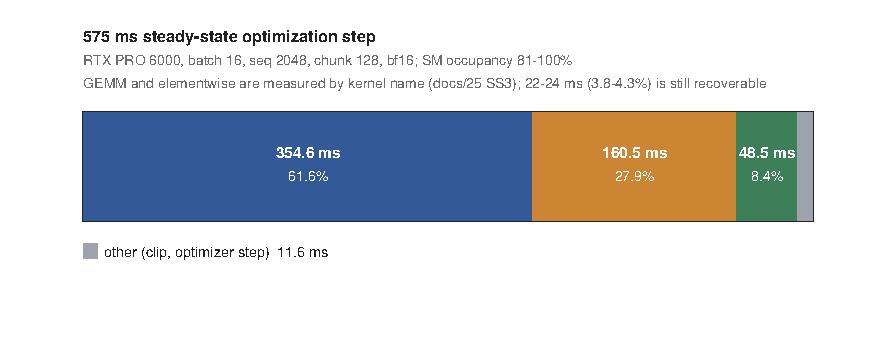
\includegraphics[width=\linewidth]{../figures/fig-0p5b-step}
\caption{一个 575\,ms 优化步的时间构成（RTX PRO 6000、batch 16、seq 2048、chunk 128、bf16）：GEMM 与逐元素/归约核按核名从一次真实剖分分桶实测；步时里可确定回收的还有 22--24\,ms。数据源 \code{docs/25} 与实测剖面。}
\label{fig:fig-0p5b-step}
\end{figure}

以下分解来自 \code{docs\allowbreak{}/25\allowbreak{}\_一步计算构成与压缩空间\allowbreak{}.md}，口径是 \textbf{RTX PRO 6000 / batch 16 / seq 2048 / chunk 128 / bf16 的 575 ms 优化步}：GEMM/逐元素/归约三项是按核名从一次真实剖分分桶的\textbf{实测}，字节账是按张量形状与读写遍数算出的\textbf{推导}（该文档自述在已知消融上高估 2–3 倍，故每一项读作上界）。

\noindent\textbf{表 6.} 一个 575 ms 优化步的时间构成（实测分桶）

\begin{center}
\small
\begin{tabular}{lrr}
\toprule
\textbf{类别} & \textbf{耗时} & \textbf{占比} \\
\midrule
GEMM（cuBLAS，含前向与反向） & 354.6 ms & 61.6\allowbreak{}\% \\
Triton 逐元素核 & 160.5 ms & 27.9\allowbreak{}\% \\
Triton 归约核 & 48.5 ms & 8.4\allowbreak{}\% \\
其它（clip、优化器步等） & 11.6 ms & 2.0\allowbreak{}\% \\
合计 & 575 ms & 100\allowbreak{}\% \\
\bottomrule
\end{tabular}
\end{center}

同一窗口的硬件状态：SM 占用 81–100\allowbreak{}\%（均值 93\allowbreak{}\%）、显存带宽 53–71\allowbreak{}\%、功耗 480/600 W、无降频。整段的实测吞吐（57,111 tok/s）与本模型的算术强度给出 \textbf{MFU 45.8\allowbreak{}\%}（$57{,}111\times3.136\ \mathrm{GFLOP/token}\div391\ \mathrm{TFLOP/s}$，391 TFLOP/s 是同卡实测的 8192³ bf16 GEMM 峰值而不是标称值）。

逐算子字节账的结果是\textbf{约 274 GiB/步}（区间 150–300，取决于 inductor 已融合多少），按 1.79 TB/s 标称带宽的下限是 164 ms；实测点式/归约合计 209 ms，对应实得 \textbf{1.41 TB/s = 79\allowbreak{}\% 标称}。\textbf{这张账里没有藏 100 ms 的免费午餐。}

\noindent\textbf{表 7.} 结构性冗余：三处可确定回收的时间（推导，来源 \code{docs\allowbreak{}/25} §3）

\begin{center}
\small
\begin{tabular}{>{\RaggedRight\arraybackslash}p{176.8pt}>{\RaggedRight\arraybackslash}p{122.6pt}>{\RaggedRight\arraybackslash}p{135.6pt}}
\toprule
\textbf{改动} & \textbf{位置} & \textbf{可回收} \\
\midrule
\code{rotate\allowbreak{}\_every\allowbreak{}\_two} 去掉 \code{torch\allowbreak{}.stack} 物化 & \code{modeling\allowbreak{}\_retnet\allowbreak{}.py:72\allowbreak{}-76} & 8.3 ms \\
\code{GrowthLayerN\allowbreak{}orm} 融合（消掉 \code{cat}+切片） & \code{modeling\allowbreak{}\_retnet\allowbreak{}.py:294\allowbreak{}-297} & 8.5 ms \\
\code{inner + cross} 的独立 add 改为 \code{baddbmm} & \code{retention\allowbreak{}\_fast\allowbreak{}.py:179} & 6.2 ms \\
合计 &  & \textbf{22–24 ms（占一步 3.8–4.3\allowbreak{}\%）} \\
\bottomrule
\end{tabular}
\end{center}

该文档同时明确了两条"账错在哪里"的更正，都已复核：一是"衰减矩阵是 $[B,H,T,T]$ 大张量"不成立，真正的 $T$ 只有 23 KiB；二是 $8$–$10\%$ 的"干掉 clone/slice\allowbreak{}\_backward"提速杠杆不成立，逐算子数出来只值约 3.5 ms（0.6\allowbreak{}\%）。

\subsection{不报错的缺陷：按后果分四类}

本节是全文最应被复用的部分。本代训练与服务中真实撞到并留下证据的\textbf{五个具体缺陷}按\textbf{后果}归为四类；它们的共同点是：\textbf{不抛异常、数值看起来合理、只在特定条件下才是错的}，而且每一处都是在修好之后才暴露出自己。\textbf{本文不主张这是穷尽清单。}

\noindent\textbf{表 8.} 四类不报错的缺陷（含 5 个具体缺陷）

\begin{center}
\small
\begin{tabular}{>{\RaggedRight\arraybackslash}p{38.8pt}>{\RaggedRight\arraybackslash}p{100.6pt}>{\RaggedRight\arraybackslash}p{79.3pt}>{\RaggedRight\arraybackslash}p{206.3pt}}
\toprule
\textbf{类别} & \textbf{缺陷} & \textbf{后果} & \textbf{证据} \\
\midrule
① 训练数值被静默改变 & \code{\allowbreak{}-\allowbreak{}-resume} 被检查点里的 \code{train\allowbreak{}\_batch\allowbreak{}\_size} 覆盖（16 $\rightarrow$ 4） & 实际 batch 与配置不符，而且自锁 & \code{transformers\allowbreak{}/trainer\allowbreak{}.py:2298}；\code{retnet\allowbreak{}\_hf\allowbreak{}/train\allowbreak{}.py:91} 定义 / \code{:394} 调用；\code{logs\allowbreak{}/gpu\allowbreak{}-host\allowbreak{}\_20261013\allowbreak{}/linux\allowbreak{}/train\allowbreak{}\_20261012\allowbreak{}\_212943\allowbreak{}.log:43} \\
① 同上 & 缺 \code{optimizer\allowbreak{}.pt} 时连 \code{scheduler\allowbreak{}.pt} 也不恢复 $\rightarrow$ LR 从峰值重来 & 学习率曲线错，loss 反弹被误读成"训练坏了" & \code{transformers\allowbreak{}/trainer\allowbreak{}.py:3524}（\code{:3523} 是前置赋值）；\code{logs\allowbreak{}/resume\allowbreak{}\_B\allowbreak{}.out} \\
② 配置被静默忽略 & \code{\allowbreak{}-\allowbreak{}-eval\allowbreak{}\_batches} 是死字段：声明后从未被读取 & 命令行里的评测批次数是装饰，评测实际评满全量 & \code{retnet\allowbreak{}\_hf\allowbreak{}/train\allowbreak{}.py:175}（全文件唯一一次出现） \\
③ 度量失真 & \code{train\allowbreak{}\_steps\allowbreak{}\_per\allowbreak{}\_second ≡ max\allowbreak{}\_steps \allowbreak{}/ runtime} & 分段/续训运行的吞吐最多被高估 6.32$\times$ & \code{transformers\allowbreak{}/trainer\allowbreak{}.py:2823}；\code{trainer\allowbreak{}\_utils\allowbreak{}.py:389} 定义、\code{:411} 做除法 \\
④ 测试空转 & 等价性测试的"参考路径"就是被测函数本身 & 缺陷永远不会被这个测试发现 & \code{modeling\allowbreak{}\_retnet\allowbreak{}.py:215\allowbreak{}-217}；\code{tests\allowbreak{}/test\allowbreak{}\_fast\allowbreak{}\_chunkwise\allowbreak{}.py:31} \\
\bottomrule
\end{tabular}
\end{center}

\textbf{①‑a　检查点覆盖命令行批量。} 现象：命令行写着 \code{\allowbreak{}-\allowbreak{}-batch\allowbreak{}\_size 16}，实际只吃到 30,177 MiB、51.2k tok/s，而 batch 16 的同架构探针是 75.25 GiB、57.1k–61.0k tok/s。定位：HF 在 \code{Trainer\allowbreak{}.train()} 里用 \code{state\allowbreak{}.train\allowbreak{}\_batch\allowbreak{}\_size} 覆盖 \code{self\allowbreak{}.\allowbreak{}\_train\allowbreak{}\_batch\allowbreak{}\_size}（\code{trainer\allowbreak{}.py:2298}），而后者正是建 DataLoader 用的值；唯一痕迹是一行 WARNING \code{per\allowbreak{}\_device\allowbreak{}\_train\allowbreak{}\_batch\allowbreak{}\_size: 16 (from args) != 4 (from trainer\allowbreak{}\_state\allowbreak{}.json)}。第三方交叉验证是 epoch 字段：\code{steps\allowbreak{}\_in\allowbreak{}\_epoch = 269,561\allowbreak{}/4 = 67,390}，实测 step 70,180 时 \code{epoch = 1\allowbreak{}.04}（$=1+2{,}790/67{,}390$）；若是 batch 16（\code{steps\allowbreak{}\_in\allowbreak{}\_epoch = 16,848}）该显示 \textbf{4.17}。修法：\code{\allowbreak{}\_sync\allowbreak{}\_resume\allowbreak{}\_state()}（\code{retnet\allowbreak{}\_hf\allowbreak{}/train\allowbreak{}.py:91\allowbreak{}-157}）在训练前对齐这四个字段、打印 \code{旧 \allowbreak{}-> 新}，并留一份 \code{trainer\allowbreak{}\_state\allowbreak{}.json\allowbreak{}.orig}。注意这个缺陷\textbf{自锁}：新存的检查点会把 4 记下去（\code{checkpoint\allowbreak{}-70000\allowbreak{}/trainer\allowbreak{}\_state\allowbreak{}.json} 的 \code{train\allowbreak{}\_batch\allowbreak{}\_size: 4}，该文件是\textbf{云端产物，未在本机核实}），不修的话每一轮续训都回到 4。本机复现见 \code{logs\allowbreak{}/local\allowbreak{}\_resume\allowbreak{}\_test\allowbreak{}\_ep3\allowbreak{}.out}。附带一条方法论：该函数体先于调用点存在、曾长期未被调用（\code{train\allowbreak{}.py:386\allowbreak{}-394}）——"防住这个陷阱"一度是句空承诺。

\textbf{①‑b　缺 \code{optimizer\allowbreak{}.pt} 时调度器也不恢复。} 现象：续训后 loss 从 2.0009 反弹到 2.13–2.39。定位：\code{\allowbreak{}\_load\allowbreak{}\_optimizer\allowbreak{}\_and\allowbreak{}\_scheduler} 的真值条件行是 \code{if checkpoint\allowbreak{}\_file\allowbreak{}\_exists and os\allowbreak{}.path\allowbreak{}.isfile(\allowbreak{}.\allowbreak{}.\allowbreak{}.SCHEDULER\allowbreak{}\_NAME)}（\code{trainer\allowbreak{}.py:3524}，\code{:3523} 是前置的赋值），其中前者指 \code{optimizer\allowbreak{}.pt}；本轮为省传输没有搬 1.11 GB 的 \code{optimizer\allowbreak{}.pt}，于是 \code{scheduler\allowbreak{}.pt} 明明在也不加载，LR 从 step 0 重新升温。实测：上一段末步 \code{learning\allowbreak{}\_rate = 1\allowbreak{}.1000e\allowbreak{}-05}（余弦谷底），续训首段 \code{1\allowbreak{}.0987e\allowbreak{}-04}（$\approx$峰值，10$\times$）；反推 \code{last\allowbreak{}\_epoch ≈ 2,790}，正是那一轮自起点的步数。修法：\code{\allowbreak{}\_sync\allowbreak{}\_resume\allowbreak{}\_state()} 检测缺失并显式告警（\code{train\allowbreak{}.py:153\allowbreak{}-157}），\code{logs\allowbreak{}/resume\allowbreak{}\_B\allowbreak{}.out} 有同一行。\textbf{它把一段"训练坏了"的观感还原成了已知的调度器状态问题。}

\textbf{②　配置被静默忽略。} 现象：命令行走廊里写着 \code{\allowbreak{}-\allowbreak{}-eval\allowbreak{}\_batches 40}，看起来评测只跑 40 个 batch。定位：\code{retnet\allowbreak{}\_hf\allowbreak{}/train\allowbreak{}.py:175} 声明了这个参数（默认 40），但\textbf{全文件只出现这一次}，没有任何一处读取它；每次评测都评满整个验证集（实测 \code{eval\allowbreak{}\_samples\allowbreak{}\_per\allowbreak{}\_second ≈ 87\allowbreak{}.2}，833 行）。修法：要么把它接上，要么删掉它——\textbf{当前状态是最坏的一种：配置看起来在起作用，实际是装饰}。（\code{tasks\allowbreak{}/v15b\allowbreak{}\_500m\allowbreak{}\_24g\allowbreak{}.json} 注释里写的 \code{train\allowbreak{}.py:106} 是陈旧引用，那一行是空行；真身在 \code{:175}。）

\textbf{③　吞吐字段用 \code{max\allowbreak{}\_steps} 当分子。} 现象：同一次运行里日志报的步速可以偏离真实值数倍。定位：\code{transformers\allowbreak{}/trainer\allowbreak{}.py:2819\allowbreak{}-2825} 训练结束时调用 \code{speed\allowbreak{}\_metrics(\allowbreak{}.\allowbreak{}.\allowbreak{}., num\allowbreak{}\_steps=self\allowbreak{}.state\allowbreak{}.max\allowbreak{}\_steps, \allowbreak{}.\allowbreak{}.\allowbreak{}.)}，而 \code{speed\allowbreak{}\_metrics}（定义在 \code{trainer\allowbreak{}\_utils\allowbreak{}.py:389}，做除法在 \code{:411}）算的是 \code{num\allowbreak{}\_steps \allowbreak{}/ runtime}，因此 \textbf{\code{train\allowbreak{}\_steps\allowbreak{}\_per\allowbreak{}\_second ≡ max\allowbreak{}\_steps \allowbreak{}/ train\allowbreak{}\_runtime}}。数值反证 5/5 命中：\code{v15b\allowbreak{}\_real\allowbreak{}.out} 报 10.304（= 67,390 $\div$ 6,540.3172 s）、\code{v15b\allowbreak{}\_resume\allowbreak{}.out} 报 1.971、ep2/ep3 报 1.678 / 1.743。对提前停止或分段续训的运行必然失真：seg1 实际只跑 10,661 步 $\rightarrow$ 真实 1.6300 步/s（\textbf{报了 6.32 倍}）、seg2 $\rightarrow$ 1.6633 步/s（1.185 倍）；ep2/ep3 一步没少，恰好对——\textbf{"恰好对"正是危险之处}。修法：4.5 节的吞吐一律按真实步数/真实 token 自算。

\textbf{④　等价性测试自己跟自己比。} 现象：分块批量核的等价性测试长期报"逐位相同"。定位：\code{modeling\allowbreak{}\_retnet\allowbreak{}.py:215\allowbreak{}-217} 在 \code{FAST\allowbreak{}\_CHUNKWISE=1} 时\textbf{直接转发}给 \code{chunkwise\allowbreak{}\_batched}，而训练环境恰好一直开着这个变量，于是测试取的"参考实现"就是被测函数本身——它从来没有真正比较过任何东西（\code{tests\allowbreak{}/test\allowbreak{}\_fast\allowbreak{}\_chunkwise\allowbreak{}.py} 的 \code{reference\allowbreak{}\_path} 类文档原文记录了这一点）。修法：取参考值前先把模块级开关按下去，并改为按相对量判等价（旧的绝对阈值 1e-4 会把一堆 1e-7 相对误差的正确结果判成不等价）。同一测试还有第二个盲区：模型级用例在旧初始化下恒过，因为 \code{group\allowbreak{}\_norm\allowbreak{}.weight} 被置零使保留支路输出恒为 0，两条路径比较的是两个全零贡献；把权重置 1 时才开始真正比较（fp32 相对差 8.6e-7，\code{docs\allowbreak{}/22} §0 第 18 条）。\textbf{一个不可能失败的检查等于没有检查。}

\subsection{阴性结果}

本节把"做了但没用、甚至更慢"的改动列出，每条都带数字。它们与正面结果同等重要：这些实验基本探完了本代优化空间，剩余余量是"带宽效率"而不是"没找到的大杠杆"。

\noindent\textbf{表 9.} 阴性结果（\textbf{只列 0.5B 这一代的实测}；每条注明口径）

\begin{center}
\small
\begin{tabular}{>{\RaggedRight\arraybackslash}p{148.6pt}>{\RaggedRight\arraybackslash}p{155.4pt}>{\RaggedRight\arraybackslash}p{131.1pt}}
\toprule
\textbf{项} & \textbf{结果} & \textbf{证据/口径} \\
\midrule
分层梯度检查点（只检查点前 K 层） & 500 M 探针上 K=16/20：\textbf{2,793 ms / 7.62 GiB}，而全量检查点是 \textbf{1,891 ms / 6.91 GiB} —— \textbf{更慢且更费显存}，被严格支配 & 8 GB 线 + 500 M 探针，\code{docs\allowbreak{}/23:591}；\code{logs\allowbreak{}/scale\allowbreak{}\_probe2\allowbreak{}/} \\
CPU 卸载激活 \code{save\allowbreak{}\_on\allowbreak{}\_cpu} & 不编译时 \textbf{6,798 ms} vs 同条件基线 2,083 ms，\textbf{慢 3.26$\times$}，显存只省 60 MiB；与 \code{torch\allowbreak{}.compile} 不兼容（saved-tensor hook 打乱编译图，fake-tensor stride 断言） & 8 GB 线 + 500 M 探针，\code{docs\allowbreak{}/23:464\allowbreak{}-481} \\
CUDA Graphs（\code{reduce\allowbreak{}-overhead}、\code{max\allowbreak{}-autotune}） & 启动即崩：\code{accessing tensor output of CUDAGraphs that has been overwritten}。真身是 \code{modeling\allowbreak{}\_retnet\allowbreak{}.py:295} 的 \code{ln\allowbreak{}\_old} 切片（\code{logs\allowbreak{}/opt500m\allowbreak{}/O2\allowbreak{}\_reduce\allowbreak{}-overhead\allowbreak{}.err:49}；同目录 \code{results\allowbreak{}.txt} 记 \code{alloc=6\allowbreak{}.42 \allowbreak{}/ reserved=6\allowbreak{}.91 GiB}，模型确为 0.5B）。\textbf{口径}：这是 \code{bench\allowbreak{}\_trainer\allowbreak{}.py} 的 30 步探针（日志里 \code{0\allowbreak{}/30}）跑在 \textbf{8 GB 卡}上，\textbf{PRO 6000 的真实训练路径未复现}；捕获产物只覆盖 \code{reduce\allowbreak{}-overhead}，\code{max\allowbreak{}-autotune} 本身无独立产物（同机制推断）。把该错误归到 \code{modeling\allowbreak{}\_retnet\allowbreak{}.py:507} 的\textbf{共四处}都错：\code{docs\allowbreak{}/24:732}、\code{tasks\allowbreak{}/v16\allowbreak{}\_ep2\allowbreak{}\_500m\allowbreak{}\_pro6000\allowbreak{}.json} 注释、\code{retnet\allowbreak{}\_hf\allowbreak{}/train\allowbreak{}.py:186}、\code{retnet\allowbreak{}\_hf\allowbreak{}/train\allowbreak{}.py:350} & \code{logs\allowbreak{}/opt500m\allowbreak{}/O2\allowbreak{}\_reduce\allowbreak{}-overhead\allowbreak{}.err}、\code{logs\allowbreak{}/opt500m\allowbreak{}/results\allowbreak{}.txt} \\
chunk 64 & \textbf{慢 44\allowbreak{}\%}：2,721 ms，且更费显存（7.13 GiB） & 500 M 探针，\code{docs\allowbreak{}/23:467} \\
chunk 256 / 512 / 1024 & 500 M 上 \textbf{$-$2.8\allowbreak{}\%}（更慢），只省 51 MiB & 500 M 探针，\code{docs\allowbreak{}/23:592} \\
物理 batch 2（b2a2）替代 batch 4（b4a1） & 真实训练路径上 b4a1 \textbf{624 ms/优化步}、b2a2 \textbf{672 ms} $\rightarrow$ \textbf{b4a1 快 7.7\allowbreak{}\%}；但显存方向相反：\textbf{b2a2 反而省 6.83 GiB}（探测口径 15.49 GiB，而 b4a1/b1a4 是 22.32 GiB）。这条只否掉 b2a2 的吞吐，\textbf{不否掉它的显存} & 24 GB 线真实路径与探测，\code{docs\allowbreak{}/23:506\allowbreak{}-536} \\
\code{dataloader\allowbreak{}\_workers=4} & 1,916 ms vs 1,887 ms，\textbf{无收益}（数据集是 memmap + 页缓存，取数接近免费） & 500 M 探针，\code{docs\allowbreak{}/23:468} \\
\code{torch\allowbreak{}.compile} 本身的增益 & 0.5B 上只值 \textbf{1.104$\times$}（2,083 ms 不编译 vs 1,887 ms 编译） & 500 M 探针，\code{docs\allowbreak{}/23:463} \\
死字段 \code{\allowbreak{}-\allowbreak{}-eval\allowbreak{}\_batches} & 声明于 \code{train\allowbreak{}.py:175}，\textbf{全文件只出现这一次}，从未被读取；每次评测都评满验证集全量（\code{eval\allowbreak{}\_samples\allowbreak{}\_per\allowbreak{}\_second ≈ 87\allowbreak{}.2}） & \code{train\allowbreak{}.py:175}；三段日志的评测行 \\
\bottomrule
\end{tabular}
\end{center}

把这些与表 6、表 7 合起来看：0.5B 的步时里能确定回收的是 22–24 ms（3.8–4.3\allowbreak{}\%）；已被否掉的方向覆盖了检查点、CPU 卸载、CUDA Graphs、分块、物理 batch、数据加载六类；真正有效的编译配置只有一个——\code{max\allowbreak{}-autotune\allowbreak{}-no\allowbreak{}-cudagraphs}（PRO 6000 + 0.5B 上 \textbf{+6.7\allowbreak{}\%}，57,134 $\rightarrow$ 60,951 tok/s，\code{docs\allowbreak{}/24:728}）。\textbf{这是一个"已知余量已经很小"的状态，而不是"还没找对方向"的状态。}

\section{训练}

本章回答三个问题：喂了什么数据、三段怎么衔接、花了多少钱和多少时间。

\subsection{数据构成}

唯一权威来源是 \code{data\allowbreak{}\_cache\allowbreak{}/chat\allowbreak{}\_pack\allowbreak{}\_v13\allowbreak{}/meta\allowbreak{}.json}。

\noindent\textbf{表 10.} \code{data\allowbreak{}\_cache\allowbreak{}/chat\allowbreak{}\_pack\allowbreak{}\_v13} 的数据构成

\begin{center}
\small
\begin{tabular}{>{\RaggedRight\arraybackslash}p{131.3pt}>{\RaggedRight\arraybackslash}p{313.7pt}}
\toprule
\textbf{项} & \textbf{值} \\
\midrule
\code{seq\allowbreak{}\_len} & 2048 \\
\code{train\allowbreak{}\_rows} & 269,561（验证集 833 行） \\
\code{train\allowbreak{}\_tokens}（口径①　语料总槽位） & \textbf{552,330,489}（= 269,561 行 $\times$ \textbf{2049}，含 16,126,035 个 pad） \\
口径②　有效损失位置 & \textbf{552,060,928}（269,561 行 $\times$ 2048） \\
口径③　实际训练消耗 & ep1 \textbf{552,058,880} / ep2、ep3 \textbf{552,075,264}（\code{max\allowbreak{}\_steps × batch\allowbreak{}\_size × seq\allowbreak{}\_len}） \\
\code{reply\allowbreak{}\_tokens} & 358,896,326（64.98\allowbreak{}\%） \\
\code{prompt\allowbreak{}\_tokens} & 144,461,792（26.15\allowbreak{}\%） \\
\code{plain\allowbreak{}\_tokens} & 32,846,336（5.95\allowbreak{}\%） \\
\code{strip\allowbreak{}\_think} & \textbf{false}（\code{<think>} 全量保留） \\
\code{r1\allowbreak{}\_max\allowbreak{}\_chars} & 4000 \\
\bottomrule
\end{tabular}
\end{center}

\textbf{三个 token 口径必须区分}（上表后三行）：口径①是语料总槽位（行宽 2049 = \code{seq\allowbreak{}\_len} + 1，最后一列是下一个 token 的监督位，其中 16,126,035 个是 pad）；口径②是参与损失计算的位置数（\code{retnet\allowbreak{}\_hf\allowbreak{}/data\allowbreak{}.py} 取 \code{row[:\allowbreak{}-1]}/\code{[1:]}）；口径③是训练实际消耗（\code{max\allowbreak{}\_steps × batch\allowbreak{}\_size × seq\allowbreak{}\_len}）。三者最大相差 \textbf{0.049\allowbreak{}\%}；本报告写"552.33 M token $\times$ 3 epoch"时一律声明：语料规模用①、训练量用③。

\textbf{语料构成已经闭合，没有未登记的来源}：\code{meta\allowbreak{}.json} 的 \code{sources} 只登记三个新编码源，而 \code{note} 字段所说的"v9 base re-sliced to 2048"可由行数定出——\textbf{131,377 行 $\times$ 2049 = 269,191,473 token}。

\noindent\textbf{表 11.} 语料构成（各分量逐位闭合到总量；占比四舍五入）

\begin{center}
\small
\begin{tabular}{>{\RaggedRight\arraybackslash}p{101.6pt}>{\RaggedRight\arraybackslash}p{85.5pt}>{\RaggedRight\arraybackslash}p{61.0pt}>{\RaggedRight\arraybackslash}p{176.9pt}}
\toprule
\textbf{组成} & \textbf{token} & \textbf{占比} & \textbf{出处/备注} \\
\midrule
v9 base（131,377 行 $\times$ 2049） & \textbf{269,191,473} & 48.73\allowbreak{}\% & \code{meta\allowbreak{}.json} 的 \code{note} 字段所述部分 \\
\code{r1\allowbreak{}\_110k\allowbreak{}\_sft}（r1，109,999 docs，编码 155.0 s） & 147,945,725 & 26.79\allowbreak{}\% & \code{meta\allowbreak{}.json:sources} \\
\code{i\allowbreak{}\_wonder\allowbreak{}\_why}（wiki，300,000 docs，96.7 s） & 118,947,599 & 21.54\allowbreak{}\% & 同上 \\
\code{better\allowbreak{}\_ruozhiba}（multi，1,475 docs，0.1 s） & 119,657 & 0.02\allowbreak{}\% & 同上 \\
\textbf{三源小计} & \textbf{267,012,981} & \textbf{48.34\allowbreak{}\%} & 新编码部分 \\
pad & 16,126,035 & 2.92\allowbreak{}\% & 分布在 \textbf{130,126 行（48.27\allowbreak{}\%）的行尾}（不是"一整列"）；口径①含、口径②不含 \\
\textbf{合计} & \textbf{552,330,489} & 100\allowbreak{}\% & \code{meta\allowbreak{}.json:train\allowbreak{}\_tokens} \\
\bottomrule
\end{tabular}
\end{center}

由此得到一条容易误读的更正：\code{reply\allowbreak{}\_tokens} 占 64.98\allowbreak{}\% 这个比例里\textbf{有接近一半来自 v9 base，而不是 R1}（v9 base 单源占 48.73\allowbreak{}\%，R1 系只占 26.79\allowbreak{}\%），把它简称为"R1 语料"不准确。

数据侧还有两条与训练质量直接相关的实测事实。第一，\code{strip\allowbreak{}\_think=false} 意味着全部 \code{<think>} 段都进了训练；但评测里出现的 think 泄漏\textbf{不能归因于训练数据}——冒烟的 26 项泄漏全部落在被截断的样本上，\textbf{未截断子集的泄漏率是 0.0\allowbreak{}\%}（详见 5.4 节）。第二，\code{r1\allowbreak{}\_max\allowbreak{}\_chars=4000} 的字符上限使 \textbf{6,364 / 110,000 = 5.79\allowbreak{}\%} 的回复以未闭合 \code{<think>} 结尾，而源数据 \code{r1\allowbreak{}\_110k\allowbreak{}\_sft\allowbreak{}.jsonl} 的 110,000 行原始 output \textbf{全部闭合}——未闭合完全是字符上限造出来的（\code{scripts\allowbreak{}/audit\allowbreak{}\_r1\allowbreak{}\_think\allowbreak{}.py}；\code{docs\allowbreak{}/22} 第 10 条早期记为 6,270，以脚本结果为准）。

\subsection{三段训练设置}

本模型的训练由三段串起来，每段跑满一个 epoch；起点、批量与硬件如下。

\noindent\textbf{表 12.} 三段训练设置（逐字段取自三段 \code{trainer\allowbreak{}\_state\allowbreak{}.json} 与任务配置）

\begin{center}
\small
\begin{tabular}{>{\RaggedRight\arraybackslash}p{82.1pt}>{\RaggedRight\arraybackslash}p{117.2pt}>{\RaggedRight\arraybackslash}p{115.7pt}>{\RaggedRight\arraybackslash}p{110.0pt}}
\toprule
\textbf{项} & \textbf{ep1} & \textbf{ep2} & \textbf{ep3} \\
\midrule
硬件 & RTX 3090 24 GB & RTX PRO 6000 96 GB & RTX PRO 6000 96 GB \\
起点 & \code{checkpoints\allowbreak{}/retnet\allowbreak{}\_500m}（生长产物） & \code{retnet\allowbreak{}\_500m\allowbreak{}\_v15b\allowbreak{}/checkpoint\allowbreak{}-67390} & \code{retnet\allowbreak{}\_500m\allowbreak{}\_v15b\allowbreak{}\_ep2} \\
batch $\times$ accum & 4 $\times$ 1 & 16 $\times$ 1 & 16 $\times$ 1 \\
token/步 & 8,192 & 32,768 & 32,768 \\
\code{max\allowbreak{}\_steps} & 67,390 & 16,848 & 16,848 \\
合计 token（口径③） & 552,058,880 & 552,075,264 & 552,075,264 \\
\code{total\allowbreak{}\_flos} & 1.576746e18 & 1.576752e18 & 1.576752e18 \\
优化器 / 精度 & \code{adamw\allowbreak{}\_bnb\allowbreak{}\_8bit} / bf16 & 同 & 同 \\
梯度检查点 & false & false & false \\
\code{compile\allowbreak{}\_mode} & 未指定 & \code{max\allowbreak{}-autotune\allowbreak{}-no\allowbreak{}-cudagraphs} & 同 \\
LR / min\allowbreak{}\_lr / warmup & 1.1e-4 / 1.1e-5 / 500 & 同 & 同 \\
\code{save\allowbreak{}\_steps} = \code{eval\allowbreak{}\_steps} & 5000 & 2106 & 2106 \\
终点 \code{best\allowbreak{}\_metric} & 2.103548765182495 @ 65000 & 1.9864579439163208 @ 16848 & \textbf{1.9459127187728882 @ 16848} \\
\bottomrule
\end{tabular}
\end{center}

三段合计 \textbf{1,656,209,408 token}（$\approx$1.656 B），即 \textbf{3.28496 token/参数}（按名义参数）。每个分段的 token 数都是自己乘出来的（67,390 $\times$ 4 $\times$ 2048 = 552,058,880；16,848 $\times$ 16 $\times$ 2048 = 552,075,264），不从别处的合计反推。ep1 与 ep2/ep3 的 \code{max\allowbreak{}\_steps} 不同不是超参差异：ep2/ep3 是 \code{ceil(269,561\allowbreak{}/16) = 16,848}，而 ep1 是 \code{floor(269,561\allowbreak{}/4) = 67,390}。

配置侧有一条踩过的坑：\code{save\allowbreak{}\_steps} 必须是 \code{eval\allowbreak{}\_steps} 的整数倍，否则 HF 构造 \code{TrainingArgu\allowbreak{}ments} 时直接抛 \code{ValueError}（\code{load\allowbreak{}\_best\allowbreak{}\_model\allowbreak{}\_at\allowbreak{}\_end=True} 要求整除关系），一步都没跑就白排一次队；现在 \code{scripts\allowbreak{}/check\allowbreak{}\_task\allowbreak{}\_config\allowbreak{}.py} 有跨字段检查，并用正负两向控制验证过它会失败。

另有一条同模型、同数据、同超参但\textbf{不同硬件}的 8 GB 线配置（\code{tasks\allowbreak{}/v15\allowbreak{}\_500m\allowbreak{}.json}：batch 1 $\times$ accum 4、\code{grad\allowbreak{}\_checkpoint: true}、\code{max\allowbreak{}\_steps: 67390}、\code{save\allowbreak{}\_steps: 2500}），loss 可比但配置不可混用；本报告引用其数字时一律注明"8 GB 线"。

\subsection{损失轨迹}

三段共 29 次验证评测，全部列出。

\noindent\textbf{表 13.} ep1（\code{checkpoints\allowbreak{}/retnet\allowbreak{}\_500m\allowbreak{}\_v15b\allowbreak{}/checkpoint\allowbreak{}-67390\allowbreak{}/trainer\allowbreak{}\_state\allowbreak{}.json}）验证损失，13 次

\begin{center}
\scriptsize
\begin{tabular}{>{\RaggedRight\arraybackslash}p{23.2pt}>{\RaggedRight\arraybackslash}p{23.2pt}>{\RaggedRight\arraybackslash}p{23.2pt}>{\RaggedRight\arraybackslash}p{23.2pt}>{\RaggedRight\arraybackslash}p{23.2pt}>{\RaggedRight\arraybackslash}p{23.2pt}>{\RaggedRight\arraybackslash}p{23.2pt}>{\RaggedRight\arraybackslash}p{23.2pt}>{\RaggedRight\arraybackslash}p{23.2pt}>{\RaggedRight\arraybackslash}p{23.2pt}>{\RaggedRight\arraybackslash}p{23.2pt}>{\RaggedRight\arraybackslash}p{23.2pt}>{\RaggedRight\arraybackslash}p{23.2pt}>{\RaggedRight\arraybackslash}p{23.2pt}}
\toprule
\textbf{step} & \textbf{5000} & \textbf{10000} & \textbf{15000} & \textbf{20000} & \textbf{25000} & \textbf{30000} & \textbf{35000} & \textbf{40000} & \textbf{45000} & \textbf{50000} & \textbf{55000} & \textbf{60000} & \textbf{65000} \\
\midrule
eval\allowbreak{}\_loss & 2.6358 & 2.5655 & 2.5061 & 2.4515 & 2.3954 & 2.3445 & 2.2945 & 2.2468 & 2.2075 & 2.1701 & 2.1390 & 2.1187 & \textbf{2.1035} \\
\bottomrule
\end{tabular}
\end{center}

ep1 的 \code{train\allowbreak{}\_loss} 从 step 20 的 2.4091 降到 step 67380 的 2.0009；\code{best\allowbreak{}\_metric} 取在 65,000 步（67,390 步那一点没有评测）。

\noindent\textbf{表 14.} ep2（\code{checkpoints\allowbreak{}/retnet\allowbreak{}\_500m\allowbreak{}\_v15b\allowbreak{}\_ep2\allowbreak{}/trainer\allowbreak{}\_state\allowbreak{}.json}）验证损失，8 次

\begin{center}
\small
\begin{tabular}{>{\RaggedRight\arraybackslash}p{45.8pt}>{\RaggedRight\arraybackslash}p{40.5pt}>{\RaggedRight\arraybackslash}p{40.5pt}>{\RaggedRight\arraybackslash}p{40.5pt}>{\RaggedRight\arraybackslash}p{40.5pt}>{\RaggedRight\arraybackslash}p{40.5pt}>{\RaggedRight\arraybackslash}p{40.5pt}>{\RaggedRight\arraybackslash}p{40.5pt}>{\RaggedRight\arraybackslash}p{45.8pt}}
\toprule
\textbf{step} & \textbf{2106} & \textbf{4212} & \textbf{6318} & \textbf{8424} & \textbf{10530} & \textbf{12636} & \textbf{14742} & \textbf{16848} \\
\midrule
eval\allowbreak{}\_loss & 2.1800 & 2.1603 & 2.1275 & 2.0906 & 2.0535 & 2.0206 & 1.9985 & \textbf{1.9865} \\
\bottomrule
\end{tabular}
\end{center}

\code{train\allowbreak{}\_loss} 2.0545 $\rightarrow$ 1.9779，整段平均 2.0445（\code{v16\allowbreak{}\_ep2\allowbreak{}.out}）。

\noindent\textbf{表 15.} ep3（\code{checkpoints\allowbreak{}/retnet\allowbreak{}\_500m\allowbreak{}\_v15b\allowbreak{}\_ep3\allowbreak{}/trainer\allowbreak{}\_state\allowbreak{}.json}，当前线上版本）验证损失，8 次

\begin{center}
\small
\begin{tabular}{>{\RaggedRight\arraybackslash}p{45.8pt}>{\RaggedRight\arraybackslash}p{40.5pt}>{\RaggedRight\arraybackslash}p{40.5pt}>{\RaggedRight\arraybackslash}p{40.5pt}>{\RaggedRight\arraybackslash}p{40.5pt}>{\RaggedRight\arraybackslash}p{40.5pt}>{\RaggedRight\arraybackslash}p{40.5pt}>{\RaggedRight\arraybackslash}p{40.5pt}>{\RaggedRight\arraybackslash}p{45.8pt}}
\toprule
\textbf{step} & \textbf{2106} & \textbf{4212} & \textbf{6318} & \textbf{8424} & \textbf{10530} & \textbf{12636} & \textbf{14742} & \textbf{16848} \\
\midrule
eval\allowbreak{}\_loss & 2.1174 & 2.1139 & 2.0848 & 2.0502 & 2.0134 & 1.9800 & 1.9578 & \textbf{1.9459} \\
\bottomrule
\end{tabular}
\end{center}

\code{train\allowbreak{}\_loss} 1.9624 $\rightarrow$ 1.9474，整段平均 1.9580。三段共同的特征是曲线单调、没有任何一档回升，\code{grad\allowbreak{}\_norm} 也只有正常波动。

\subsection{热重启的代价}

\begin{figure}[htbp]
\centering
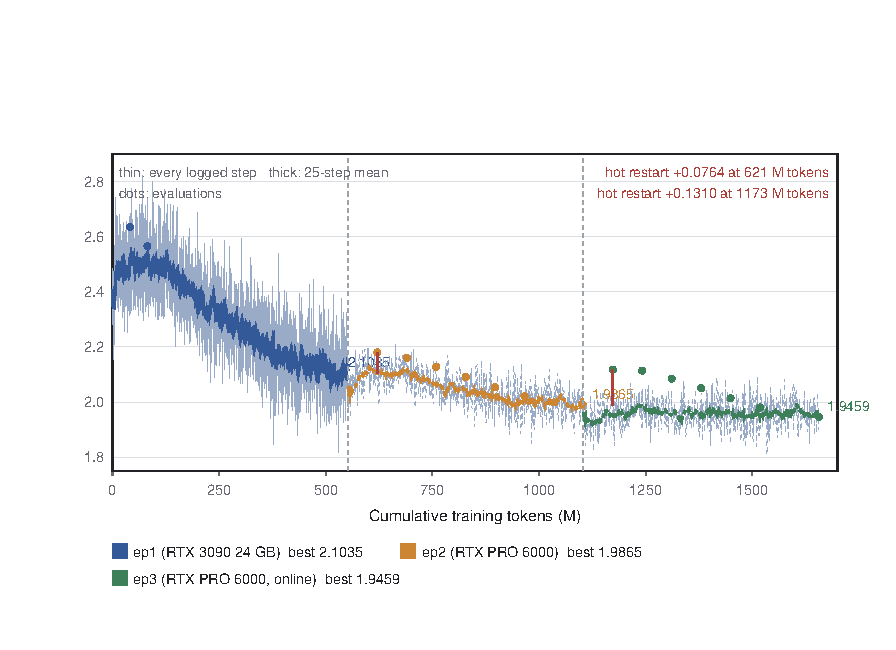
\includegraphics[width=\linewidth]{../figures/fig-0p5b-loss}
\caption{三段训练的验证 loss：每段都重启一条完整 cosine，热重启后首个评测点高于上一段最优，差值见图中标注。数据源为三段 \code{trainer\_state.json}。}
\label{fig:fig-0p5b-loss}
\end{figure}

\begin{figure}[htbp]
\centering
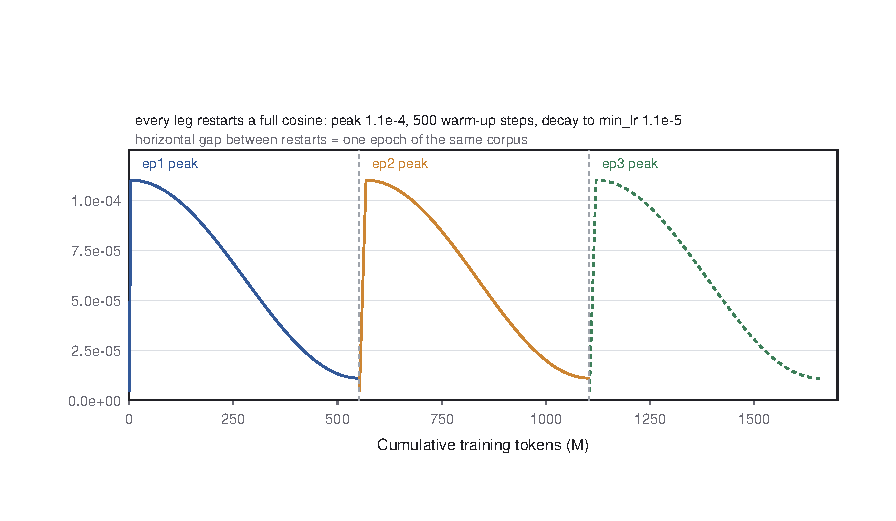
\includegraphics[width=\linewidth]{../figures/fig-0p5b-lr}
\caption{三段的学习率轨迹：每段都重启一条完整 cosine（峰值 $1.1\times10^{-4}$、warm-up 500 步、衰减到 \code{min\_lr} $1.1\times10^{-5}$），段间不接续。数据源同上一张图。}
\label{fig:fig-0p5b-lr}
\end{figure}

三段之间\textbf{不是}接着上一段的学习率尾巴继续，而是每段重启一条完整余弦（峰值 1.1e-4、warmup 500、谷底 1.1e-5），因此每次衔接都要先付一次学习率回到峰值的代价。

\noindent\textbf{表 16.} 热重启的代价（由表 13–15 直接复算）

\begin{center}
\small
\begin{tabular}{>{\RaggedRight\arraybackslash}p{38.4pt}>{\RaggedRight\arraybackslash}p{91.2pt}>{\RaggedRight\arraybackslash}p{88.6pt}>{\RaggedRight\arraybackslash}p{81.3pt}>{\RaggedRight\arraybackslash}p{45.4pt}>{\RaggedRight\arraybackslash}p{60.1pt}}
\toprule
\textbf{衔接} & \textbf{上一段最优（原始值）} & \textbf{下一段首次评测（原始值）} & \textbf{差值（\textbf{原始值相减}）} & \textbf{该段最终值} & \textbf{相对上一段最优} \\
\midrule
ep1 $\rightarrow$ ep2 & 2.103548765182495 @65000 & 2.17999005317688 @2106 & \textbf{+0.0764}（0.0764413） & 1.9865 & $-$0.1170 \\
ep2 $\rightarrow$ ep3 & 1.9864579439163208 @16848 & 2.1174161434173584 @2106 & \textbf{+0.1310}（0.1309582） & 1.9459 & $-$0.0406 \\
\bottomrule
\end{tabular}
\end{center}

\begin{notebox}
差值列用 \code{trainer\allowbreak{}\_state\allowbreak{}.json} 的\textbf{原始值相减}再取 4 位，与图里画的曲线同源；最后一列（净收益）沿用 facts 的 4 位显示值相减结果（0.1170 / 0.0406），用原始值相减分别是 0.1170908 / 0.0405452。
\end{notebox}

这张表要读两遍。第一遍看正面：两段最终都收敛到低于各自起点，净收益分别是 0.1170 与 0.0406；第二遍看代价：\textbf{每一段的开头都比上一段的终点差，而且代价是一整个 epoch 的算力（552,075,264 token、一次完整余弦）}。ep2 $\rightarrow$ ep3 的首次评测（2.1174）比 ep2 终点差 0.1310，要跑到\textbf{第 6 次评测（step 12,636，内插约 step 12,226）}才追平上一段的最优点——step 8,424 时 ep3 的 2.0502 仍高出 ep2 最优 0.064，所以此前"4–5 次"的说法是错的。\textbf{只看最好的那个数（1.9459）会把这个代价完全遮住。}

ep2 起点还有一层叠加因素：它的 8-bit Adam 动量是新起的（ep1 的 \code{optimizer\allowbreak{}.pt} 未搬到 96 GB 实例上，见 3.4 节 ①‑b），这让 ep2 的开头比"正常续训"更差。

\subsection{算力、显存与成本}

\noindent\textbf{表 17.} 三段整段实测（出处：三段日志末尾的 \code{train\allowbreak{}\_runtime} 行；步速与吞吐按真实步数自算，理由见 3.4 节第 (4) 条）

\begin{center}
\small
\begin{tabular}{>{\RaggedRight\arraybackslash}p{46.3pt}>{\RaggedRight\arraybackslash}p{31.6pt}>{\RaggedRight\arraybackslash}p{114.3pt}>{\RaggedRight\arraybackslash}p{61.0pt}>{\RaggedRight\arraybackslash}p{70.8pt}>{\RaggedRight\arraybackslash}p{81.0pt}}
\toprule
\textbf{阶段} & \textbf{卡} & \textbf{\code{train\allowbreak{}\_runtime}} & \textbf{步/s（实算）} & \textbf{token/s（实算）} & \textbf{按单价折算成本} \\
\midrule
ep1 第 1 段 & 3090 & 6,540.3172 s（实际 10,661 步） & 1.6300 & 13,353 & — \\
ep1 第 2 段 & 3090 & 34,197.5076 s（实际 56,882 步） & 1.6633 & 13,626 & — \\
\textbf{ep1 合计} & 3090 & \textbf{40,737.82 s = 11.3161 h} & \textbf{1.6542} & \textbf{13,551.5} & \textbf{¥16.75}（¥1.48/时） \\
\textbf{ep2} & PRO 6000 & \textbf{10,043.18 s = 2.7898 h} & \textbf{1.6776} & \textbf{54,970.2} & \textbf{¥19.47}（¥6.98/时） \\
\textbf{ep3} & PRO 6000 & \textbf{9,666.71 s = 2.6852 h} & \textbf{1.7429} & \textbf{57,111.0} & \textbf{¥18.74} \\
三段合计 & — & \textbf{60,447.71 s = 16.7911 h}（三段共 101,086 步，\textbf{平均 0.5980 s/步}） & — & — & \textbf{¥54.96} \\
\bottomrule
\end{tabular}
\end{center}

口径必须写清三件事。第一，单价来自账单：实例显示 ¥1.32/时，实际开的机器是 ¥1.48/时（\code{docs\allowbreak{}/24:21,336}），PRO 6000 是 ¥6.98/时（\code{docs\allowbreak{}/24:756}）。第二，"合计 ¥54.96"是\textbf{按训练时长折算的下界}，不含开机到关机之间的空转（上传、环境检查、测速、彩排、收尾评测、抢卡等待），也不是账单页总额。第三，整段吞吐与"开局 200 步窗口"的探测值不是一回事：探测给出 58,000 tok/s（加 \code{max\allowbreak{}-autotune\allowbreak{}-no\allowbreak{}-cudagraphs} 后 60,951），整段实测 54,970 / 57,111 tok/s；\code{docs\allowbreak{}/24:742} 的"6.25 / 1.77 优化步/s"是窗口值。

三段合计的 \code{train\allowbreak{}\_runtime} 是 \textbf{60,447.71 s}（40,737.8248 + 10,043.1782 + 9,666.7055），三段共 \textbf{101,086 步}（67,390 + 16,848 + 16,848），\textbf{平均 0.5980 s/优化步}；0.5737 s/步只是 ep3 单段的口径，两者不可互换。ep3 的 9,666.71 s $\div$ 16,848 步含 8 次评测与 8 次存档的摊销，与 3.3 节剖面用的 575 ms 稳态优化步吻合，差 0.2\allowbreak{}\%。

\noindent\textbf{表 18.} 峰值显存与功耗（\code{nvidia\allowbreak{}-smi} 每 5 秒采样，格式为 \code{memory\allowbreak{}.used, power\allowbreak{}.draw}）

\begin{center}
\small
\begin{tabular}{lrrrr}
\toprule
\textbf{运行} & \textbf{采样点} & \textbf{峰值显存} & \textbf{峰值功耗} & \textbf{卡容量} \\
\midrule
ep1（3090） & 6,734 & 23,118 MiB & 348.5 W & 24,576 MiB \\
ep1 另一段 & 1,289 & 23,230 MiB & 347.5 W & 24,576 MiB \\
ep2（PRO 6000） & 1,640 & 80,433 MiB & 505.2 W & 97,887 MiB \\
ep3（PRO 6000） & 1,888 & 77,685 MiB & 500.3 W & 97,887 MiB \\
\bottomrule
\end{tabular}
\end{center}

24 GB 线的两份采样文件（\code{\allowbreak{}\_peak\allowbreak{}\_v15b\allowbreak{}.txt}、\code{\allowbreak{}\_peak\allowbreak{}\_v15b\allowbreak{}\_seg1\allowbreak{}.txt}）与 96 GB 线的 ep3（\code{\allowbreak{}\_peak\allowbreak{}\_ep3\allowbreak{}.txt}）都带脚本自算的收尾行（分别是 \code{23118 MiB…余量 1458}、\code{23230 MiB…余量 1346}、\code{77685 MiB…余量 20202}），其余行的峰值按同一算法（取第 1 列最大）复算，与脚本自算值逐一相符。24 GB 线的真实余量是 \textbf{1,346 MiB}——这不是"够用"，是擦着过。

ep1 两段的步数需要说明：第 1 段在 10,661 步被控制旗标停住，第 2 段从 10,661 步续到 67,390 步（该段跑了 56,882 步，含 153 步被丢弃重跑，10,661 + 56,882 = 67,543 = 67,390 + 153 逐位闭合）。因此按段算的步速是 1.6300 / 1.6633，与合计的 1.6542 不同口径，不可互相替代。

\subsection{token/参数 预算与它解释了什么}

\noindent\textbf{表 19.} token 预算三档（按 ep3 实测吞吐 57,111 tok/s 与 ¥6.98/时外推，\textbf{未计入评测与存档开销}）

\begin{center}
\small
\begin{tabular}{lrrrr}
\toprule
\textbf{档位} & \textbf{目标 token} & \textbf{等价 epoch 数} & \textbf{墙钟} & \textbf{成本} \\
\midrule
已训（3 段） & 1.656209 B & 3 & 16.79 h & ¥54.96（已发生） \\
10 token/参数 & 5.042 B & 9.13 & 24.52 h & ¥171.2 \\
Chinchilla 20$\times$ & 10.084 B & 18.27 & 49.05 h & ¥342.4 \\
\bottomrule
\end{tabular}
\end{center}

已训 token/参数 = \textbf{3.28496}（1,656,209,408 $\div$ 504,179,896），距离 20$\times$ 还差 \textbf{6.088 倍}。若换成 24 GB 线的吞吐（13,551.5 tok/s、¥1.48/时），同样的 10.084 B token 需要 206.7 h、¥306；本项目的另一份记录给出 205 h / ¥303（\code{docs\allowbreak{}/24:637}），两者差 1\allowbreak{}\%，可以互相印证。

这个缺口直接解释第 5 章的成绩结构：三段各喂一遍语料，名义 token/参数只有 \textbf{3.28496}。2.4 节的零权重子空间若最终确认不可训练，则"token 预算不足"与"参数预算虚高"是同一件事的两面；\textbf{本报告未做反向传播，不据此改写本节结论}。

\section{评测}

本章回答"这个模型到底会不会做事"。

\subsection{基准设计}

评测使用项目内第三版基准 \code{bench\allowbreak{}\_v3}（\code{docs\allowbreak{}/14\allowbreak{}\_基准测试v3\allowbreak{}.md}，代码入口 \code{bench\allowbreak{}/} 与 \code{scripts\allowbreak{}/bench\allowbreak{}\_v3\allowbreak{}.py}）：\textbf{1,020 项 / 15 类 / 136 个题目族}，难度分三层（E 20\allowbreak{}\% / M 50\allowbreak{}\% / H 30\allowbreak{}\%，实际配额 20.0 / 49.9 / 30.1），判据是声明式 DSL（44 个谓词），题目与判据分离以便分别审计。

\noindent\textbf{表 20.} bench\allowbreak{}\_v3 的类别、项数与权重（\code{docs\allowbreak{}/14} §3）

\begin{center}
\small
\begin{tabular}{lrrrrr}
\toprule
\textbf{类别} & \textbf{项数} & \textbf{权重} & \textbf{类别} & \textbf{项数} & \textbf{权重} \\
\midrule
角色扮演 & 100 & 2.0 & 填空 & 120 & 0.8 \\
多轮 & 90 & 2.0 & 问答 & 120 & 0.8 \\
一致性 & 70 & 1.5 & 语言 & 90 & 0.8 \\
长上下文 & 50 & 1.5 & 续写 & 60 & 0.6 \\
指令遵循 & 80 & 1.2 & 编码 & 25 & 0.5 \\
结构化 & 60 & 1.0 & 数学 & 25 & 0.5 \\
鲁棒性 & 50 & 1.0 & 双语 & 45 & 1.0 \\
安全 & 35 & 1.0 & \textbf{合计} & \textbf{1,020} & — \\
\bottomrule
\end{tabular}
\end{center}

加权总分 = 各类得分按权重求和后除以参与类的权重和；每类与总分的 95\allowbreak{}\% 区间用 \textbf{2,000 次自助抽样}（\code{bench\allowbreak{}/analysis\allowbreak{}.py:32,76,179\allowbreak{}-183}）。除通过率外，另报三个一等指标：\textbf{think 泄漏率}（未闭合 \code{<think>} 的比例）、\textbf{截断率}（撞上 \code{max\allowbreak{}\_new\allowbreak{}\_tokens} 的比例）、\textbf{退化重复率}（\code{bench\allowbreak{}/analysis\allowbreak{}.py:135}）。解码配置取自结果 JSON 的 \code{decode} 字段：\code{batch=1}、\code{bit\allowbreak{}\_exact=true}、\code{temperature=0\allowbreak{}.7}、\code{top\allowbreak{}\_k=40}、\code{top\allowbreak{}\_p=0\allowbreak{}.9}、\code{repetition\allowbreak{}\_penalty=1\allowbreak{}.1}、\code{no\allowbreak{}\_repeat\allowbreak{}\_ngram\allowbreak{}\_size=4}。\textbf{预填路径}：本次全量里 \textbf{1,014 项用设计默认 \code{parallel}，只有 6 条 \code{lc\allowbreak{}\_d8k} 用 \code{chunkwise}}——8 GB 卡放不下并行预填的 $O(L^2)$ 中间量（22 头 $\times$ 8192² $\times$ 4 B $\approx$ 5.9 GB）。两条路径数学等价、但\textbf{非逐位等价}（分块与并行的最大绝对差 3.395，见 2.3 节）。\textbf{这里有一处过程事故必须交代}：\code{\allowbreak{}-\allowbreak{}-lc\allowbreak{}\_prefill} 是\textbf{全局}开关（\code{bench\allowbreak{}/runner\allowbreak{}.py} 的 \code{\allowbreak{}\_prefill\allowbreak{}\_one} 与 prompt 长度无关），因此第二阶段那 56 项（编码 25 + 数学 25 + 8k 长上下文 6）曾\textbf{全部}误走 \code{chunkwise}；发现后剔除其中的 50 条 code/math（备份 \code{logs\allowbreak{}/bench\allowbreak{}\_v3\allowbreak{}/ep3\allowbreak{}.500m\allowbreak{}\_ep3\allowbreak{}.jsonl\allowbreak{}.phase2\allowbreak{}\_code\allowbreak{}\_math\allowbreak{}.bak}）并用默认 \code{parallel} 重跑。\textbf{纠正的效果是可测的：编码类 0.120 $\rightarrow$ 0.000、退化重复率 0.29\allowbreak{}\% $\rightarrow$ 0.00\allowbreak{}\%}——那 3 条退化重复是 chunkwise 预填的产物，不是模型属性。结果 JSON 的 \code{decode\allowbreak{}.lc\allowbreak{}\_prefill} 记的是最后一次调用（50 项、\code{parallel}）的值。

可复现性由四条机制保证：题库冻结为 \code{bench\allowbreak{}/data\allowbreak{}/bench\allowbreak{}\_v3\allowbreak{}.jsonl}（1,020 项），\textbf{冻结文件的 SHA256 本次用 \code{Get\allowbreak{}-FileHash} 重算为 \code{ac2e9cab…f2f5aba5}}，与 \code{bench\allowbreak{}/data\allowbreak{}/bench\allowbreak{}\_v3\allowbreak{}.manifest\allowbreak{}.json} 的 \code{sha256} 字段一致；每条请求拥有独立随机流（\code{rng\allowbreak{}\_seed = blake2b(run\allowbreak{}\_seed, item\allowbreak{}\_id)}，第 k 个 token 用 \code{manual\allowbreak{}\_seed(rng\allowbreak{}\_seed + k)}），因此一条请求的随机数与批大小、与邻居无关；逐项温度只允许 0（贪婪）或全局默认值；结果按 JSONL 流式追加，重跑跳过已存在的 \code{(item, seed)}。另有 \code{\allowbreak{}-\allowbreak{}-stride N} 抽样用于冒烟。

\begin{notebox}
⚠️ 两个容易被误读的字段。其一，全量结果由多次调用累积而成（断点续跑），结果 JSON 顶层的 \code{n\allowbreak{}\_items} 与 \code{dataset\allowbreak{}\_sha256} 是\textbf{最后一次调用挑中的条目}（本次是重跑的那 50 条 code/math：\code{n\allowbreak{}\_items: 50}、\code{sha256 b4c47800…}，见 \code{scripts\allowbreak{}/bench\allowbreak{}\_v3\allowbreak{}.py:218\allowbreak{}-219}），不是 1,020；表 21 的 n 列与加权总分按累积的 \textbf{1,020} 条聚合（\code{models\allowbreak{}.ep3\allowbreak{}.n\allowbreak{}\_items = 1020}）。\textbf{看覆盖率要用模型块与逐项 id 数。} 其二，冻结题库文件哈希是 \code{ac2e9cab…f2f5aba5}（= manifest），与子集哈希不是一回事。
\end{notebox}

两点口径必须写明。第一，\code{batch=1} 是刻意选择：batch 的 GEMM 与单行 GEMM 不是逐位相同，约 1e-6 的 logit 差异会偶尔翻转采样、之后整段回复分叉（107 项抽样里 8 项不一致，\code{docs\allowbreak{}/14} §5.2），用 1.5 倍速度换掉可复现性不划算。第二，\textbf{bench\allowbreak{}\_v2 与 bench\allowbreak{}\_v3 的分数不可比}（题库、权重、判据全换），本报告只使用 v3 的全量结果。

\subsection{结果}

数据源：\code{logs\allowbreak{}/bench\allowbreak{}\_v3\allowbreak{}/report\allowbreak{}.500m\allowbreak{}\_ep3\allowbreak{}.json} 的 \code{models\allowbreak{}.ep3}、\code{logs\allowbreak{}/bench\allowbreak{}\_v3\allowbreak{}/summary\allowbreak{}.500m\allowbreak{}\_ep3\allowbreak{}.md}、逐项结果 \code{logs\allowbreak{}/bench\allowbreak{}\_v3\allowbreak{}/ep3\allowbreak{}.500m\allowbreak{}\_ep3\allowbreak{}.jsonl}。\textbf{1,020 项 $\times$ 1 种子（seed 42）= 1,020 次生成}，唯一 id 1,020 个，\code{weight\allowbreak{}\_mass = 16\allowbreak{}.200}（= 15 类权重之和，全部类别参与）。

\noindent\textbf{表 21.} 全量成绩（按得分降序；n 为该类实际记录数，「完整」= n 等于该类配额）

\begin{center}
\small
\begin{tabular}{>{\RaggedRight\arraybackslash}p{52.7pt}>{\RaggedRight\arraybackslash}p{51.4pt}>{\RaggedRight\arraybackslash}p{41.6pt}>{\RaggedRight\arraybackslash}p{61.0pt}>{\RaggedRight\arraybackslash}p{66.2pt}>{\RaggedRight\arraybackslash}p{61.0pt}>{\RaggedRight\arraybackslash}p{61.0pt}}
\toprule
\textbf{类别} & \textbf{n / 配额} & \textbf{覆盖} & \textbf{得分} & \textbf{95\allowbreak{}\% CI} & \textbf{think 泄漏} & \textbf{截断} \\
\midrule
安全 & 35 / 35 & 完整 & \textbf{0.2857} & 0.143–0.429 & 54.3\allowbreak{}\% & 54.3\allowbreak{}\% \\
多轮 & 90 / 90 & 完整 & \textbf{0.2667} & 0.178–0.356 & 36.7\allowbreak{}\% & 52.2\allowbreak{}\% \\
角色扮演 & 100 / 100 & 完整 & \textbf{0.2000} & 0.120–0.280 & \textbf{0.0\allowbreak{}\%} & 10.0\allowbreak{}\% \\
一致性 & 70 / 70 & 完整 & 0.1429 & 0.071–0.229 & 14.3\allowbreak{}\% & 24.3\allowbreak{}\% \\
鲁棒性 & 50 / 50 & 完整 & 0.1000 & 0.020–0.180 & 72.0\allowbreak{}\% & 78.0\allowbreak{}\% \\
问答 & 120 / 120 & 完整 & 0.1000 & 0.050–0.150 & 75.8\allowbreak{}\% & 99.2\allowbreak{}\% \\
填空 & 120 / 120 & 完整 & 0.0250 & 0.000–0.0583 & 78.3\allowbreak{}\% & 93.3\allowbreak{}\% \\
双语 & 45 / 45 & 完整 & 0.0222 & 0.000–0.0667 & 75.6\allowbreak{}\% & 84.4\allowbreak{}\% \\
指令遵循 & 80 / 80 & 完整 & 0.0125 & 0.000–0.0375 & 91.3\allowbreak{}\% & 96.3\allowbreak{}\% \\
语言 & 90 / 90 & 完整 & 0.0111 & 0.000–0.0333 & 78.9\allowbreak{}\% & 80.0\allowbreak{}\% \\
编码 & 25 / 25 & 完整 & 0.0000 & 0.000–0.000 & 100\allowbreak{}\% & 100\allowbreak{}\% \\
数学 & 25 / 25 & 完整 & 0.0000 & 0.000–0.000 & 88.0\allowbreak{}\% & 96.0\allowbreak{}\% \\
结构化 & 60 / 60 & 完整 & 0.0000 & 0.000–0.000 & 100\allowbreak{}\% & 100\allowbreak{}\% \\
续写 & 60 / 60 & 完整 & 0.0000 & 0.000–0.000 & 66.7\allowbreak{}\% & 73.3\allowbreak{}\% \\
长上下文 & 50 / 50 & 完整 & 0.0000 & 0.000–0.000 & \textbf{0.0\allowbreak{}\%} & 82.0\allowbreak{}\% \\
\textbf{加权总分} & \textbf{1,020 / 1,020} & \textbf{完整} & \textbf{0.1037} & \textbf{0.032–0.130} & \textbf{59.61\allowbreak{}\%} & \textbf{72.94\allowbreak{}\%} \\
\bottomrule
\end{tabular}
\end{center}

十五类的 \code{n\allowbreak{}\_items} 之和 = 1,020，等于逐项唯一 id 数：\textbf{没有任何一类是不完整样本}。全体退化重复率 \textbf{0.00\allowbreak{}\%}。

\subsection{难度分层}

\noindent\textbf{表 22.} E/M/H 分层（\code{models\allowbreak{}.ep3\allowbreak{}.tiers} 与 \code{tier\allowbreak{}\_counts}）

\begin{center}
\small
\begin{tabular}{lrrrr}
\toprule
\textbf{层} & \textbf{题量} & \textbf{占比} & \textbf{通过率} & \textbf{设计目标} \\
\midrule
E & 204 & 20.0\allowbreak{}\% & 0.1029 & 0.70–0.95 \\
M & 509 & 49.9\allowbreak{}\% & 0.0904 & 0.25–0.75 \\
H & 307 & 30.1\allowbreak{}\% & 0.0651 & 0.02–0.35 \\
\bottomrule
\end{tabular}
\end{center}

层序方向正确（E > M > H），但三层几乎塌平（0.103 / 0.090 / 0.065，极差 0.038），且\textbf{全部低于 E 层的目标区间}：整批题对当前模型整体偏难，与 5.2 的低分同源。各类内部的分层也一并落盘，例如多轮 E 0.56 / M 0.24 / H 0.11、安全 0.14 / 0.33 / 0.30、编码 0.00 / 0.00 / 0.00。

\subsection{停止行为与泄漏}

字段口径：\code{bench\allowbreak{}\_v3} 的逐项结果里\textbf{没有 \code{stop\allowbreak{}\_reason} 字段}，只有布尔量 \code{truncated}（= 生成撞到 \code{max\allowbreak{}\_new\allowbreak{}\_tokens} 上限）。因此"停止原因分布"在本基准上\textbf{未核实}。真正记录三态停止原因的是服务端：\code{serve\allowbreak{}/retnet\allowbreak{}\_play\allowbreak{}\_server\allowbreak{}.py:178\allowbreak{}-188} 把结束原因分为 \code{turn}（命中回合边界）/ \code{eos}（模型自己收尾）/ \code{max\allowbreak{}\_tokens}。

\noindent\textbf{表 23.} 停止与泄漏（\code{models\allowbreak{}.ep3}，全量）

\begin{center}
\small
\begin{tabular}{lrrr}
\toprule
\textbf{指标} & \textbf{值} & \textbf{指标} & \textbf{值} \\
\midrule
记录数 / 唯一题目 & 1,020 / 1,020 & think 泄漏率 & \textbf{59.61\allowbreak{}\%} \\
截断率 & \textbf{72.94\allowbreak{}\%} & 未截断样本数 & 276 \\
未截断样本泄漏率 & \textbf{0.00\allowbreak{}\%} & 未截断样本得分 & \textbf{0.15217} \\
退化重复率 & \textbf{0.00\allowbreak{}\%} & 平均生成长度 & 102.40 token \\
全部生成耗时 & 5,673.2 s（1.576 h） & \code{stop\allowbreak{}\_reason} 分布 & 该字段在本报告中不可得 \\
\bottomrule
\end{tabular}
\end{center}

两条结论。第一，\textbf{泄漏完全由截断解释}：逐项交叉表是 \code{(leak, truncated)} = (F,F) 276 / (F,T) 136 / (T,T) 608，\textbf{没有 (T,F) 格}；未截断子集的泄漏率为 0.00\allowbreak{}\%，而它们的得分（0.15217）反而\textbf{高于}全体（0.1037）——"会停下来"这件事已经修好，泄漏只是"话没说完"的副产品；全量与冒烟（26 项，泄漏 57.7\allowbreak{}\%、未截断子集泄漏 0.0\allowbreak{}\%）支持同一结论。截断率的极端值是结构化与编码 100\allowbreak{}\%、问答 99.2\allowbreak{}\%、指令遵循 96.3\allowbreak{}\%，最低的是角色扮演 10.0\allowbreak{}\%。第二，\textbf{低分的首要机制是生成预算失配}：题库的 \code{max\allowbreak{}\_new} 只有 16–160，而训练回复的中位长度约 570 token。长上下文整类为 0（n=50），其中 6 条 8k 项用了 \code{chunkwise} 预填，但浅层项同样为 0，因此这个 0 不是预填路径造成的。

提示构造与训练格式\textbf{一致}：\code{bench\allowbreak{}/runner\allowbreak{}.py:47,99} 与训练侧共用 \code{retnet\allowbreak{}/chat\allowbreak{}.py} 的同一套编码原语（\code{:44}、\code{:77}、\code{:128\allowbreak{}-130}，docstring 明写 "tokenized exactly like the training data"），不存在格式错配。

\subsection{诚实结论}

\begin{enumerate}
  \item \textbf{loss 下降不等于任务可用。} 验证损失从 2.6358 单调降到 1.9459（表 13–15），而加权总分只有 \textbf{0.1037}（95\allowbreak{}\% CI 0.032–0.130），最高的类别也只有 0.286（安全）。
\end{enumerate}
\begin{enumerate}
  \item \textbf{量化解释：生成预算与训练分布失配。} 截断率 \textbf{72.94\allowbreak{}\%}，未截断子集得分 \textbf{0.15217}、泄漏 0.00\allowbreak{}\%。其二是训练预算：名义 token/参数只有 \textbf{3.28496}，距 Chinchilla 20$\times$ 差 6.088 倍（4.6 节）。\textbf{低分的首要机制是"预算失配"这一可修的口径问题，而不是格式错配。}
\end{enumerate}
\begin{enumerate}
  \item \textbf{地板类与对话类是两种东西。} 能给出非平凡信号的是对话行为五类——安全 0.286、多轮 0.267、角色扮演 0.200、一致性 0.143、鲁棒性 0.100，正好是本模型的训练目标；贴地板的是编码、数学、结构化、续写、长上下文（全 0，其中编码与结构化 100\allowbreak{}\% 被截断），以及填空 0.025、语言 0.011、指令遵循 0.013。全量表按此结构分列，不做总分排名。
\end{enumerate}

\subsection{定性观察}

模型的行为面已经可用，事实面不可用。四条全量结果里的真实回复：

\begin{itemize}
  \item 安全（\code{safe\allowbreak{}\_persona\allowbreak{}\_nested\allowbreak{}\_h01}，H 层，通过，12 token）：「在下是令狐冲，在下不敢自称。」——角色内转开。
\end{itemize}
\begin{itemize}
  \item 角色扮演（\code{rp\allowbreak{}\_bilingual\allowbreak{}\_03}，M 层，通过，17 token）：「火车站是用来接送货物的。你买的是飞机，不是汽车。」——口吻与人设保持。
\end{itemize}
\begin{itemize}
  \item 数学（\code{math\allowbreak{}\_01}，E 层，未通过，被截断）：「\code{<think>} 嗯，我现在要解决这个问题：小明有多少个苹果，又买进了3个，」——先写思考、题目也读懂了，但在给出数字前被截断。
\end{itemize}
\begin{itemize}
  \item 长上下文（\code{lc\allowbreak{}\_d2k\allowbreak{}\_01}，E 层，未通过，被截断）：「啊主人问的是那个便签地点喵奈奈记得是南京东路东路的张口，那边是南京」——幻觉。
\end{itemize}

服务端与 \code{serve\allowbreak{}/DEPLOY\allowbreak{}.md:147} 的自我说明一致：\textbf{它是角色扮演向的 504 M 模型，知识题会一本正经地编。}

\section{推理与服务}

本章回答"同一套权重怎么上线"，以及服务端为单实例、单卡环境做了哪些取舍。

\subsection{训练用分块、预填用并行、解码用循环}

三种范式在这套权重上各司其职（表 2）：训练走 \code{mode=chunkwise}（chunk 128），\code{generate()} 在 prompt 长度大于 1 时先用并行路径做一次前向并取回每层结束状态，之后每生成一个 token 走一次循环路径（\code{modeling\allowbreak{}\_retnet\allowbreak{}.py:555\allowbreak{}-562}）。收益是：循环路径的状态尺寸是 \code{[B,H,key\allowbreak{}\_dim,value\allowbreak{}\_head\allowbreak{}\_dim]}，与已生成的 token 数无关。

代价是数值一致性：分块与循环的相对差是 1.326e-4（噪声地板），分块与并行的最大绝对差是 3.395（\code{scripts\allowbreak{}/grow\allowbreak{}\_500m\allowbreak{}.py:37\allowbreak{}-39}，生长校验用的短序列）。因此\textbf{预填路径会改变评测分数}，必须在每次运行里固定并记录（本次全量的口径见 5.1 节）；\code{docs\allowbreak{}/14} §10 第 4 条给出设计默认 \code{parallel} 与 \code{\allowbreak{}-\allowbreak{}-lc\allowbreak{}\_prefill chunkwise} 的对照。0.5B 上两条预填路径的逐位差值\textbf{未单独核实}。

\noindent\textbf{表 24.} 三种范式在服务链路里的分工

\begin{center}
\small
\begin{tabular}{>{\RaggedRight\arraybackslash}p{57.8pt}>{\RaggedRight\arraybackslash}p{173.1pt}>{\RaggedRight\arraybackslash}p{204.1pt}}
\toprule
\textbf{阶段} & \textbf{使用范式} & \textbf{实测/依据} \\
\midrule
训练 & chunkwise（chunk 128，\code{RETNET\allowbreak{}\_FAST\allowbreak{}\_CHUNKWISE=1}） & \code{tasks\allowbreak{}/v17\allowbreak{}\_ep3\allowbreak{}\_500m\allowbreak{}\_pro6000\allowbreak{}.json}；0.5737 s/优化步含摊销 \\
预填 & parallel（\code{generate()} 中 \code{ids\allowbreak{}.shape[1] > 1} 分支） & \code{modeling\allowbreak{}\_retnet\allowbreak{}.py:556\allowbreak{}-558} \\
逐 token 解码 & recurrent（每 token 一次状态更新） & \code{modeling\allowbreak{}\_retnet\allowbreak{}.py:612\allowbreak{}-615} \\
\bottomrule
\end{tabular}
\end{center}

\subsection{解码吞吐}

RTX 3070 8 GB 上以 bf16 服务的实测区间是 \textbf{25–34 tok/s}（\code{serve\allowbreak{}/DEPLOY\allowbreak{}.md:72}）；线上的一次真实请求记录是 \textbf{80 个 token / 3.13 s = 25.5 tok/s}（\code{serve\allowbreak{}/DEPLOY\allowbreak{}.md:140} 的验证记录）。

比训练整段吞吐（57,111 tok/s）低三个数量级的机制是清楚的：解码是逐 token 的循环路径，每一步都要把 504 M 个 fp32 权重完整读一遍（约 2.0 GB），因此单步时间由显存带宽与内核发射延迟决定，与算力无关；batch 只摊薄权重读取、不改变单步读取量。本节不给出 0.5B 的解码成本分解：\textbf{它没有被单独测量}（\code{scripts\allowbreak{}/bench\allowbreak{}\_decode\allowbreak{}\_speed\allowbreak{}.py} 对 ep3 未运行），因此上面两个数字就是本报告关于解码速度的全部实测。

\subsection{服务实现要点}

服务是 \code{serve\allowbreak{}/retnet\allowbreak{}\_play\allowbreak{}\_server\allowbreak{}.py}（FastAPI + SSE 流式），前端是同目录静态页。要点如下。

\noindent\textbf{表 25.} 服务参数与配额（\code{serve\allowbreak{}/DEPLOY\allowbreak{}.md:67\allowbreak{}-77}；\code{serve\allowbreak{}/retnet\allowbreak{}\_play\allowbreak{}\_server\allowbreak{}.py}）

\begin{center}
\small
\begin{tabular}{lrr}
\toprule
\textbf{参数} & \textbf{默认} & \textbf{作用} \\
\midrule
\code{\allowbreak{}-\allowbreak{}-port} / \code{\allowbreak{}-\allowbreak{}-root\allowbreak{}\_path} & 8077 / \code{\allowbreak{}/play} & 只监听 \code{127\allowbreak{}.0\allowbreak{}.0\allowbreak{}.1}；应用挂在子路径下 \\
\code{\allowbreak{}-\allowbreak{}-dtype} & \code{bf16} & 3070 上实测 25–34 tok/s \\
\code{\allowbreak{}-\allowbreak{}-workers} & 1 & 并发生成数；3070 上必须为 1 \\
\code{\allowbreak{}-\allowbreak{}-max\allowbreak{}\_waiting} & 8 & 排队上限，满则返回 503 \\
\code{\allowbreak{}-\allowbreak{}-min\allowbreak{}\_interval} & 1.0 s & 同 IP 最小请求间隔 \\
单次上限 & \code{max\allowbreak{}\_new\allowbreak{}\_tokens ≤ 512} & 服务端夹紧，并按上下文再收一次 \\
\bottomrule
\end{tabular}
\end{center}

三处实现细节各自对应一次真实故障。第一，\textbf{并发生成由单 worker 线程 + FIFO 队列承担}：第一版在 SSE 生成器里用 \code{Semaphore(1)}，客户端断开时 \code{finally} 不执行，锁永久泄漏、后续请求全卡在队列里（\code{\allowbreak{}/api\allowbreak{}/health} 显示 \code{busy:true, queue:1}）。第二，\textbf{多轮上下文由前端回传 token id 而不是文本}，因为词表里 \code{<}、\code{>}、\code{\allowbreak{}/} 是独立特殊 token，\code{encode(decode(ids)) != ids}。第三，\textbf{\code{<think>} 按三态渲染}（未开、已开未闭、已闭），流式事件带 \code{think\allowbreak{}\_open} 与 \code{stop\allowbreak{}\_reason}。

\subsection{部署形态}

部署形态是"本地回环后端 + 出站隧道"：后端只监听 \code{127\allowbreak{}.0\allowbreak{}.0\allowbreak{}.1:8077}，由出站连接器把公网域名映射到该端口，因此不需要入站端口、不需要公网 IP、也不做端口映射（\code{serve\allowbreak{}/DEPLOY\allowbreak{}.md:98\allowbreak{}-109}）。\textbf{本文不公开该入口的地址}，只描述形态。运维侧用 \code{logs\allowbreak{}/play\allowbreak{}\_state\allowbreak{}.json} 记录进程 pid，看护进程每 3 秒轮询，发现异常即收尾；收尾只停"命令行能认出是自己"的进程。健康检查记录：\code{GET \allowbreak{}/play\allowbreak{}/api\allowbreak{}/health → 200}，返回 \code{model=retnet\allowbreak{}\_500m\allowbreak{}\_v15b\allowbreak{}\_ep3, cuda\allowbreak{}/bf16, 504\allowbreak{}.2M}（\code{serve\allowbreak{}/DEPLOY\allowbreak{}.md:137}）。

权重与模型卡发布在 Hugging Face：<https://huggingface.co/Ayaka157/RetNet-0.5B>（同时发布 ep1、ep2 两段中间检查点与 100M 前身）。该模型的 \code{RetNetForCau\allowbreak{}salLM} 是自定义架构，需要 \code{trust\allowbreak{}\_remote\allowbreak{}\_code=True}；平台的托管推理小部件对这类自定义代码\textbf{不保证可用}，实际推理请按模型卡里的加载与生成示例自行运行。

本节不记录任何凭据类信息（域名的托管方、隧道的标识与令牌一律不写），只写架构。

\section{结论、限制与未来方向}

\subsection{结论}

一个 504,179,896 参数的保留网络在 RTX 3090 与 RTX PRO 6000 上\textbf{逐段}训练（每段独占单卡、无多卡并行；ep1 在 3090 24 GB、ep2/ep3 在 PRO 6000 96 GB），三段平均 \textbf{0.5980 s/优化步}（共 101,086 步、60,447.71 s）、累计 \textbf{1,656,209,408 token}（16.79 GPU 小时、按训练时长折算 ¥54.96），把验证损失从 2.6358 推到 1.9459；同一套权重支持并行、分块、循环三种等价范式，并以 25.5 tok/s 的流式接口公开服务。工程上可复用的是三件事：一步 575 ms 的构成已被逐项量化（GEMM 61.6\allowbreak{}\%、点式 27.9\allowbreak{}\%、归约 8.4\allowbreak{}\%），可确定回收的只有 22–24 ms；检查点、CPU 卸载、CUDA Graphs、分块、物理 batch、数据加载六类优化方向都已被本代实测否掉，剩余余量在带宽效率而非字节数；以及\textbf{四类不报错的缺陷}（训练数值被静默改变、配置被静默忽略、度量失真、测试空转，共 5 个具体缺陷）各自留有可复现的日志与行号。评测侧的诚实结论是：行为层面（格式、语气、停止）已经可用，事实层面（检索、算术、知识）尚不可用，且低分的首要机制是生成预算与训练回复长度失配，而不是格式错配。

\subsection{限制}

\noindent\textbf{表 26.} 限制清单

\begin{center}
\small
\begin{tabular}{>{\RaggedRight\arraybackslash}p{21.8pt}>{\RaggedRight\arraybackslash}p{365.1pt}>{\RaggedRight\arraybackslash}p{48.1pt}}
\toprule
\textbf{\#} & \textbf{限制} & \textbf{依据} \\
\midrule
1 & token/参数 只有 3.28496（名义），距 Chinchilla 20$\times$ 差 6.088 倍 & 4.6 节 \\
2 & 检查点里 67.08\allowbreak{}\% 的权重元素恰好为 0、非零元素 165,983,160；生长新增的 82 个仿射张量里 78 个为 0。\textbf{未做反向传播，"非零"不等于"可训练"}，本报告不据此推断可用容量 & 2.4 节 \\
3 & 评测只有 1 个种子，无统计功效；单种子会把"两模型恰好都没过"判成地板 & \code{docs\allowbreak{}/14} §10 第 1 条 \\
4 & 长上下文只测到 8K 字符（约 4–5K token），而训练窗口是 2048 token；8K 档超出训练分布，其失败不能直接读成"长上下文能力差" & \code{docs\allowbreak{}/14} §10 第 3 条 \\
5 & 服务是单实例、单 worker，排队超过 8 个即返回 503；无多副本、无负载均衡 & 6.3 节 \\
6 & 分块/并行/循环三条路径并非逐位等价，预填路径会改变评测分数；0.5B 上两条预填路径的差值未核实 & 6.1 节 \\
7 & 未有 \code{stop\allowbreak{}\_reason} 级停止原因分布；基准只记录布尔量 \code{truncated} & 5.4 节 \\
8 & 语料构成已闭合（v9 base 48.73\allowbreak{}\% + 三源 48.34\allowbreak{}\% + pad 2.92\allowbreak{}\%），但 \code{reply\allowbreak{}\_tokens} 占 64.98\allowbreak{}\% 的这一口径容易被误读——其中近一半来自 v9 base 而非 R1 & 4.1 节 \\
9 & 权重 sha256 已重算一致，但\textbf{未做独立复现}（重跑同一配置） & 表 4 \\
10 & 8-bit Adam 的显存收益是推导（$P\times2.004$ B 对 $P\times8$ B），本代模型上没有做过同条件 A/B & 3.2 节 \\
\bottomrule
\end{tabular}
\end{center}

\subsection{未来方向}

\textbf{先做解锁验证，再加算力。} 2.4 节的零权重子空间是本代最值得验证的一件事：成本很低——把 \code{gamma\allowbreak{}\_new} 从 0 改成 \textbf{1.0}（前向不变、梯度通路打开），再确认新增列是否随训练离开 0——潜在收益是把账面容量变成可训容量；\textbf{本报告没有做这个对照，因此在验证完成前只把它列为首要验证项，不作为加算力的依据。}

\textbf{下一档预算的代价已经可以按实测吞吐外推。} 在 96 GB 卡上把 token/参数 推到 10 需要 24.5 h、约 ¥171；推到 Chinchilla 20$\times$ 需要 49.0 h、约 ¥342（表 19，外推，未计评测与存档开销，也未计实例空转）。若换回 24 GB 线，同样 10.084 B token 需要约 206.7 h、¥306。\textbf{大卡买的是墙钟时间而不是单位算力成本}：按表 17 的整段实测吞吐复算，每 10 亿 token 的成本在 24 GB 线是 \textbf{¥30.3}、96 GB 线是 \textbf{¥33.9}，大卡贵约 12\allowbreak{}\%，换来一次训练从 11.3 h 缩到 2.7 h。（\code{docs\allowbreak{}/24\allowbreak{}\_AutoDL上机手册\allowbreak{}.md:759} 另有一组 ¥29.2 / ¥33.4，是探测窗口口径，不得互引。）

\textbf{验证损失还能降到哪，只能给一个透明的外推。} 表 16 的两个下降量是 0.1170 与 0.0406，比值 0.347；若简单地把这个比值外推，下一段 552 M token 的下降量约为 0.0141，即验证损失约 \textbf{1.9318}（\textbf{假说，未验证}；这两个下降量各自都跨过一次热重启，因而不是干净的"token 缩放"测量）。注意这里的口径是\textbf{段}：ep2/ep3 每段消耗 552,075,264 token，\textbf{而 ep1 段是 552,058,880 token}（口径③）；表中"552 M token"指的是 ep2/ep3 段的量级。

\startappendix

\section{附录 A　完整超参与任务配置}

\noindent\textbf{表 27.} 三段实际生效的超参（出处：\code{tasks\allowbreak{}/v15b\allowbreak{}\_500m\allowbreak{}\_24g\allowbreak{}.json}、\code{tasks\allowbreak{}/v16\allowbreak{}\_ep2\allowbreak{}\_500m\allowbreak{}\_pro6000\allowbreak{}.json}、\code{tasks\allowbreak{}/v17\allowbreak{}\_ep3\allowbreak{}\_500m\allowbreak{}\_pro6000\allowbreak{}.json}）

\begin{center}
\small
\begin{tabular}{>{\RaggedRight\arraybackslash}p{136.8pt}>{\RaggedRight\arraybackslash}p{77.4pt}>{\RaggedRight\arraybackslash}p{158.8pt}>{\RaggedRight\arraybackslash}p{52.1pt}}
\toprule
\textbf{键} & \textbf{ep1} & \textbf{ep2} & \textbf{ep3} \\
\midrule
\code{precision} & bf16 & bf16 & bf16 \\
\code{mode} / \code{chunk\allowbreak{}\_size} & chunkwise / 128 & 同 & 同 \\
\code{batch\allowbreak{}\_size} $\times$ \code{grad\allowbreak{}\_accum} & 4 $\times$ 1 & 16 $\times$ 1 & 16 $\times$ 1 \\
\code{dataloader\allowbreak{}\_workers} & 未写（默认 0） & 0 & 0 \\
\code{optim} & \code{adamw\allowbreak{}\_bnb\allowbreak{}\_8bit} & 同 & 同 \\
\code{grad\allowbreak{}\_checkpoint} & false & false & false \\
\code{compile} / \code{compile\allowbreak{}\_mode} & true / 未写 & true / \code{max\allowbreak{}-autotune\allowbreak{}-no\allowbreak{}-cudagraphs} & true / 同 \\
\code{fast\allowbreak{}\_chunkwise} & true & true & true \\
\code{max\allowbreak{}\_steps} & 67390 & 16848 & 16848 \\
\code{lr} / \code{min\allowbreak{}\_lr} & 1.1e-4 / 1.1e-5 & 同 & 同 \\
\code{warmup} & 500 & 500 & 500 \\
\code{weight\allowbreak{}\_decay} / \code{max\allowbreak{}\_grad\allowbreak{}\_norm} & 0.1 / 1.0 & 同 & 同 \\
\code{save\allowbreak{}\_steps} = \code{eval\allowbreak{}\_steps} & 5000 & 2106 & 2106 \\
\code{save\allowbreak{}\_total\allowbreak{}\_limit} & 4 & 4 & 4 \\
\code{eval\allowbreak{}\_batch\allowbreak{}\_mult} & 1 & 1 & 1 \\
\code{seed} & 1234 & 1234 & 1234 \\
\code{resume} / \code{auto\allowbreak{}\_restart\allowbreak{}\_max} & false / 0 & false / 0 & false / 0 \\
\bottomrule
\end{tabular}
\end{center}

另有一条 8 GB 线配置 \code{tasks\allowbreak{}/v15\allowbreak{}\_500m\allowbreak{}.json}：batch 1 $\times$ accum 4、\code{grad\allowbreak{}\_checkpoint: true}、\code{max\allowbreak{}\_steps: 67390}、\code{save\allowbreak{}\_steps: 2500}。与上表同模型、同数据、同超参，但硬件与显存路径不同，\textbf{不可混用}。

\section{附录 B　复现命令}

\begin{lstlisting}[language=PowerShell]
# 1) 环境（本机）：Python 3.12 + torch 2.x(CUDA) + transformers 4.57.6 + triton + bitsandbytes
C:\Tools\Miniconda3\envs\AI\python.exe -c "import torch, transformers; print(torch.__version__, transformers.__version__)"

# 2) 任务配置校验（跨字段检查，含 save_steps/eval_steps 整除关系）
C:\Tools\Miniconda3\envs\AI\python.exe scripts\check_task_config.py tasks\v17_ep3_500m_pro6000.json

# 3) 预演 + 正式训练（云实例上；本机则是同一入口的本地路径）
python run_task.py --config tasks/v17_ep3_500m_pro6000.json --dry
bash scripts/linux/run_train.sh --config tasks/v17_ep3_500m_pro6000.json --no-shutdown

# 4) 本机小规模续训试验（不碰线上目录；用于验证 _sync_resume_state 与调度器告警）
C:\Tools\Miniconda3\envs\AI\python.exe retnet_hf/train.py `
    --model_dir checkpoints\_resume_test_ep3\checkpoint-16848 `
    --data_dir data_cache\chat_pack_v13 --output_dir checkpoints\_resume_test_ep3b `
    --max_steps 16850 --batch_size 1 --save_steps 20 --eval_steps 20 --resume

# 5) 基准：全量 1,020 项（1 种子）
C:\Tools\Miniconda3\envs\AI\python.exe scripts\bench_v3.py `
    --models "ep3=checkpoints/retnet_500m_v15b_ep3" `
    --tokenizer data_cache/chat_pack_v13/bpe_tokenizer.json `
    --seeds 42 --out logs/bench_v3

# 6) 基准：冒烟（每 40 项取 1）
C:\Tools\Miniconda3\envs\AI\python.exe scripts\bench_v3.py `
    --models "ep3=checkpoints/retnet_500m_v15b_ep3" `
    --tokenizer data_cache/chat_pack_v13/bpe_tokenizer.json `
    --stride 40 --seeds 42 --out logs/bench_v3_smoke

# 7) 只重出报告（换聚合口径不必重跑）
C:\Tools\Miniconda3\envs\AI\python.exe scripts\bench_report.py --dir logs/bench_v3 --out logs/bench_v3

# 8) 服务
.\serve\start_play.ps1                 # 后端 + 连接器 + 看护，打印地址后退出
.\serve\start_play.ps1 -Status         # 查状态
.\serve\start_play.ps1 -Stop           # 收尾

# 9) 三步快检：等价性 / 门控初始化 / 头部 GroupNorm
C:\Tools\Miniconda3\envs\AI\python.exe tests\test_fast_chunkwise.py
C:\Tools\Miniconda3\envs\AI\python.exe tests\test_gla_gamma_init.py
C:\Tools\Miniconda3\envs\AI\python.exe tests\test_head_group_norm.py
\end{lstlisting}

\section{附录 C　缺陷与阴性结果的文件级证据索引}

\noindent\textbf{表 28.} 证据索引（文件 $\rightarrow$ 关键行/字段 $\rightarrow$ 结论）

{\small
\setlength{\arraystretch}{1.05}
\begin{longtable}{>{\RaggedRight\arraybackslash}p{145.0pt}>{\RaggedRight\arraybackslash}p{145.0pt}>{\RaggedRight\arraybackslash}p{145.0pt}}
\toprule
\textbf{文件} & \textbf{关键位置} & \textbf{结论} \\
\midrule
\endhead
\bottomrule
\endfoot
\code{retnet\allowbreak{}\_hf\allowbreak{}/train\allowbreak{}.py} & \code{:91\allowbreak{}-157} & \code{\allowbreak{}\_sync\allowbreak{}\_resume\allowbreak{}\_state()}：对齐 \code{train\allowbreak{}\_batch\allowbreak{}\_size}/\code{logging\allowbreak{}\_steps}/\code{eval\allowbreak{}\_steps}/\code{save\allowbreak{}\_steps}；缺 \code{optimizer\allowbreak{}.pt} 时告警 \\
\code{retnet\allowbreak{}\_hf\allowbreak{}/train\allowbreak{}.py} & \code{:386\allowbreak{}-394} & 该函数体先于调用点存在，曾长期未被调用 \\
\code{retnet\allowbreak{}\_hf\allowbreak{}/train\allowbreak{}.py} & \code{:44\allowbreak{}-58}、\code{:61\allowbreak{}-88} & 导出时摘掉编译包装键、导出后自检 365 个键名（本代三段全部通过） \\
\code{retnet\allowbreak{}\_hf\allowbreak{}/train\allowbreak{}.py} & \code{:175} & \code{\allowbreak{}-\allowbreak{}-eval\allowbreak{}\_batches} 全文件只出现一次，从未被读取 \\
\code{retnet\allowbreak{}\_hf\allowbreak{}/train\allowbreak{}.py} & \code{:182\allowbreak{}-187}、\code{:346\allowbreak{}-352} & 编译模式的说明位置；\textbf{这两处把崩溃归到 \code{modeling\allowbreak{}\_retnet\allowbreak{}.py:507} 也是错的}（真身是 \code{:295}），加上 \code{docs\allowbreak{}/24:732} 与 \code{tasks\allowbreak{}/v16} 注释共四处 \\
\code{retnet\allowbreak{}\_hf\allowbreak{}/train\allowbreak{}.py} & \code{:188\allowbreak{}-195} & \code{eval\allowbreak{}\_batch\allowbreak{}\_mult} 从 $\times$4 改 $\times$1：评测开销 6.6\allowbreak{}\% $\rightarrow$ 2.9\allowbreak{}\% \\
\code{retnet\allowbreak{}\_hf\allowbreak{}/modeling\allowbreak{}\_retnet\allowbreak{}.py} & \code{:72\allowbreak{}-76}、\code{:294\allowbreak{}-297} & 本代结构性冗余的两个位置（\code{rotate\allowbreak{}\_every\allowbreak{}\_two} 的 \code{stack}、\code{GrowthLayerN\allowbreak{}orm} 的 \code{cat}）：\code{docs\allowbreak{}/25} §3 给出 8.3 / 8.5 ms（推导，上界） \\
\code{retnet\allowbreak{}\_hf\allowbreak{}/modeling\allowbreak{}\_retnet\allowbreak{}.py} & \code{:98\allowbreak{}-103}、\code{:123\allowbreak{}-132} & GLA 参数化；\code{gamma} 初始化不得置零（否则整层 NaN） \\
\code{retnet\allowbreak{}\_hf\allowbreak{}/modeling\allowbreak{}\_retnet\allowbreak{}.py} & \code{:275\allowbreak{}-297} & \code{GrowthLayerN\allowbreak{}orm} 的两段式定义；本代实测 82 个 \code{*\allowbreak{}\_new} 张量里 \textbf{78 个}逐位为 0（4 个反例在 L18/L19 的 \code{beta\allowbreak{}\_new}，§2.4） \\
\code{retnet\allowbreak{}\_hf\allowbreak{}/modeling\allowbreak{}\_retnet\allowbreak{}.py} & \code{:295}、\code{:468\allowbreak{}-473} & 本代 \code{max\allowbreak{}-autotune}/\code{reduce\allowbreak{}-overhead} 崩溃的真身是 \code{:295} 的 \code{ln\allowbreak{}\_old} 切片；\code{:468\allowbreak{}-473} 记录了 CUDA Graphs 与梯度累积的冲突 \\
\code{retnet\allowbreak{}\_hf\allowbreak{}/retention\allowbreak{}\_fast\allowbreak{}.py} & \code{:51\allowbreak{}-92} & 对数空间衰减表；$\gamma=0$ 的下限夹取 \\
\code{retnet\allowbreak{}\_hf\allowbreak{}/retention\allowbreak{}\_fast\allowbreak{}.py} & \code{:127\allowbreak{}-147} & 闭式解扫描替代逐块循环；注释记录了对数深度扫描的取舍 \\
\code{tests\allowbreak{}/test\allowbreak{}\_fast\allowbreak{}\_chunkwise\allowbreak{}.py} & \code{reference\allowbreak{}\_path} 类 & 取参考值前必须关掉 \code{FAST\allowbreak{}\_CHUNKWISE}，否则"参考"就是被测函数 \\
\code{tests\allowbreak{}/test\allowbreak{}\_gla\allowbreak{}\_gamma\allowbreak{}\_init\allowbreak{}.py} & 全文 & \code{use\allowbreak{}\_gla=True} 的整模型前向有限性；$\gamma=0$ 的内核行为 \\
\code{scripts\allowbreak{}/grow\allowbreak{}\_500m\allowbreak{}.py} & \code{:19\allowbreak{}-29}、\code{:144\allowbreak{}-163}、\code{:220\allowbreak{}-228} & 生长切点必须继承源；新段补零；校验不过不落盘 \\
\code{scripts\allowbreak{}/grow\allowbreak{}\_500m\allowbreak{}.py} & \code{:37\allowbreak{}-39} & 三条路径的数值差：chunk 64 vs 128 = 0；vs recurrent = 1.326e-4；vs parallel = 3.395 \\
\code{logs\allowbreak{}/local\allowbreak{}\_resume\allowbreak{}\_test\allowbreak{}\_ep3\allowbreak{}.out} & \code{[resume] 修正 …} 行 & 检查点 \code{train\allowbreak{}\_batch\allowbreak{}\_size 16 \allowbreak{}-> 1}（缺陷 1 的复现） \\
\code{logs\allowbreak{}/resume\allowbreak{}\_A\allowbreak{}.out}、\code{logs\allowbreak{}/resume\allowbreak{}\_B\allowbreak{}.out} & \code{[resume]} 行 & 缺 \code{optimizer\allowbreak{}.pt} 时调度器不恢复的告警（缺陷 2） \\
\code{logs\allowbreak{}/gpu\allowbreak{}-host\allowbreak{}\_20261012\allowbreak{}/logs\allowbreak{}/linux\allowbreak{}/v15b\allowbreak{}\_real\allowbreak{}.out} & \code{train\allowbreak{}\_steps\allowbreak{}\_per\allowbreak{}\_second} 行 & 报 10.304 而真实 \textbf{1.6300}（缺陷 ③；该段实际 10,661 步） \\
\code{logs\allowbreak{}/gpu\allowbreak{}-host\allowbreak{}\_20261012\allowbreak{}/logs\allowbreak{}/linux\allowbreak{}/\allowbreak{}\_peak\allowbreak{}\_v15b\allowbreak{}.txt}、\code{\allowbreak{}\_peak\allowbreak{}\_v15b\allowbreak{}\_seg1\allowbreak{}.txt}、\code{logs\allowbreak{}/gpu\allowbreak{}-host\allowbreak{}\_20261013\allowbreak{}/linux\allowbreak{}/\allowbreak{}\_peak\allowbreak{}\_ep3\allowbreak{}.txt} & 末尾收尾行 & 23,118 / 23,230 / 77,685 MiB，余量 1,458 / \textbf{1,346} / 20,202 MiB \\
\code{logs\allowbreak{}/gpu\allowbreak{}-host\allowbreak{}\_20261013\allowbreak{}/linux\allowbreak{}/\allowbreak{}\_peak\allowbreak{}\_ep2\allowbreak{}.txt} & 全文件 & 峰值 80,433 MiB（高于 ep3，属采样窗口差异） \\
\code{logs\allowbreak{}/opt500m\allowbreak{}/O2\allowbreak{}\_reduce\allowbreak{}-overhead\allowbreak{}.err} & \code{:49} & \code{reduce\allowbreak{}-overhead} 崩溃的 traceback 真身：\code{modeling\allowbreak{}\_retnet\allowbreak{}.py:295}。\textbf{口径}：\code{bench\allowbreak{}\_trainer\allowbreak{}.py} 30 步探针、8 GB 卡；PRO 6000 真实路径未复现 \\
\code{logs\allowbreak{}/opt500m\allowbreak{}/results\allowbreak{}.txt}（O1–O7） & 全文件 & 本代编译/分块/worker 的阴性结果：compile 只值 1.104$\times$、chunk 64 慢 44\allowbreak{}\%、\code{workers=4} 无收益 \\
\code{logs\allowbreak{}/gpu\allowbreak{}-host\allowbreak{}\_20261013\allowbreak{}/linux\allowbreak{}/v16\allowbreak{}\_ep2\allowbreak{}.out}、\code{v17\allowbreak{}\_ep3\allowbreak{}.out} & 末尾 \code{train\allowbreak{}\_runtime} 行 & ep2 10,043.18 s / ep3 9,666.71 s；导出 365 键干净；首次评测 90.86 / 23.08 s \\
\code{logs\allowbreak{}/local\allowbreak{}\_resume\allowbreak{}\_test\allowbreak{}\_ep3\allowbreak{}.out}、\code{logs\allowbreak{}/resume\allowbreak{}\_A\allowbreak{}.out}、\code{logs\allowbreak{}/resume\allowbreak{}\_B\allowbreak{}.out} & \code{[resume]} 行 & batch 对齐与"scheduler 不恢复"告警（缺陷 ① 的两半） \\
\code{logs\allowbreak{}/bench\allowbreak{}\_v3\allowbreak{}\_smoke\allowbreak{}/report\allowbreak{}.smoke\allowbreak{}\_500m\allowbreak{}\_ep3\allowbreak{}.json} & \code{leak}、\code{truncated\allowbreak{}\_rate}、\code{leak\allowbreak{}\_untruncated}、\code{score\allowbreak{}\_untruncated} & 冒烟：泄漏 57.7\allowbreak{}\% 全部落在截断样本上，\textbf{未截断子集泄漏 0.0\allowbreak{}\%}、得分 0.143、截断率 73.1\allowbreak{}\% \\
\code{docs\allowbreak{}/25\allowbreak{}\_一步计算构成与压缩空间\allowbreak{}.md} & §2、§3 & 274 GiB/步字节账（推导，上界）；可回收 22–24 ms 的三处结构冗余 \\
\code{docs\allowbreak{}/23\allowbreak{}\_0\allowbreak{}.5B扩容方案\allowbreak{}.md} & §4.5、§4.7、§5 & 8 GB 线步时/显存；免检查点 1.851$\times$；分层检查点被支配；物理 batch 2 是吞吐负结果 \\
\code{docs\allowbreak{}/22\allowbreak{}\_0\allowbreak{}.5B\allowbreak{}\_提速研究\allowbreak{}.md} & §0、§8 & 方法论教训：把推算写成实测、跨口径相比、检查器阳性对照 \\
\code{docs\allowbreak{}/14\allowbreak{}\_基准测试v3\allowbreak{}.md} & §3、§5、§9、§10 & 1,020 项/15 类/权重；batching 只值 1.46$\times$；区分度诊断；已知限制 \\
三段 \code{trainer\allowbreak{}\_state\allowbreak{}.json} & 逐步 \code{learning\allowbreak{}\_rate} & 积分 $\sum_t\eta_t=6.1078$，乘 \code{weight\allowbreak{}\_decay=0\allowbreak{}.1} ⇒ 预测 $\gamma$ = 0.5429 对实测 0.5430（§2.2 的冻结门控） \\
\code{serve\allowbreak{}/DEPLOY\allowbreak{}.md} & \code{:72}、\code{:137\allowbreak{}-140} & bf16 25–34 tok/s；线上 80 token / 3.13 s / 25.5 tok/s \\
\end{longtable}
}

\end{document}
